\documentclass{ntuthesis}

\usepackage{times}
\usepackage{verbatim}
\usepackage{color}
\usepackage{url}
\usepackage{graphicx}
\usepackage{array}
\usepackage{wallpaper}
\usepackage{hyperref}
\usepackage[printwatermark]{xwatermark}
\usepackage{graphicx}
\usepackage{pdfpages}
\usepackage{enumitem}

% Using the tex-text mapping for ligatures etc.
\defaultfontfeatures{Mapping=tex-text}

% Set the default fonts
\setmainfont{Times New Roman}
\setCJKmainfont{BiauKai}

\ifdefined\withwatermark
  \newwatermark*[allpages,xpos=6.1725cm,ypos=10.5225cm,scale=0.5]{
\includegraphics{watermark.pdf}}
\fi

% digital object identifier
\ifdefined\withdoi
  \insertdoi
\fi

\makeatletter
\AtBeginDocument{
  \hypersetup{
    pdftitle={\@titleen},
    pdfauthor={\@authoren},
    pdfsubject={\@typeen{} \@classen},
    pdfkeywords={\@keywordsen}
  }
}
\makeatother

% Your information goes here
% author: Tz-Huan Huang [http://www.csie.ntu.edu.tw/~tzhuan]

% ----------------------------------------------------------------------------
% "THE CHOCOLATE-WARE LICENSE":
% Tz-Huan Huang wrote this file. As long as you retain this notice you
% can do whatever you want with this stuff. If we meet some day, and you think
% this stuff is worth it, you can buy me a chocolate in return Tz-Huan Huang
% ----------------------------------------------------------------------------

% Syntax: \var{English}{Chinese}
\university{National Taiwan University}{國立臺灣大學}
\college{College of Electrical Engineering and Computer Science}{電機資訊學院}
\institute{Graduate Institute of Communication Engineering}{電信工程學研究所}
\title{FileFarm: A Secured Cloud-of-Clouds Storage System}{FileFarm: 安全的雲中雲儲存系統}
\author{Yu-Ping Huang}{黃宇平}
\studentid{R06942065}
\advisor{Tsung-Nan Lin, Ph.D.}{林宗男 博士}
\defenseyear{2019}{108}
\defensemonth{July}{7}
\defenseday{24}
\doi{10.6342/NTU201902637}
\keywords{Cloud Storage, Cloud-of-Clouds, MultiCloud, DHT, Kademlia, P2P Storage}{雲端儲存、雲中雲、分散式雜湊表、Kademlia、端對端儲存}


\begin{document}

\frontmatter

\makecover

\ifdefined\withcertification
  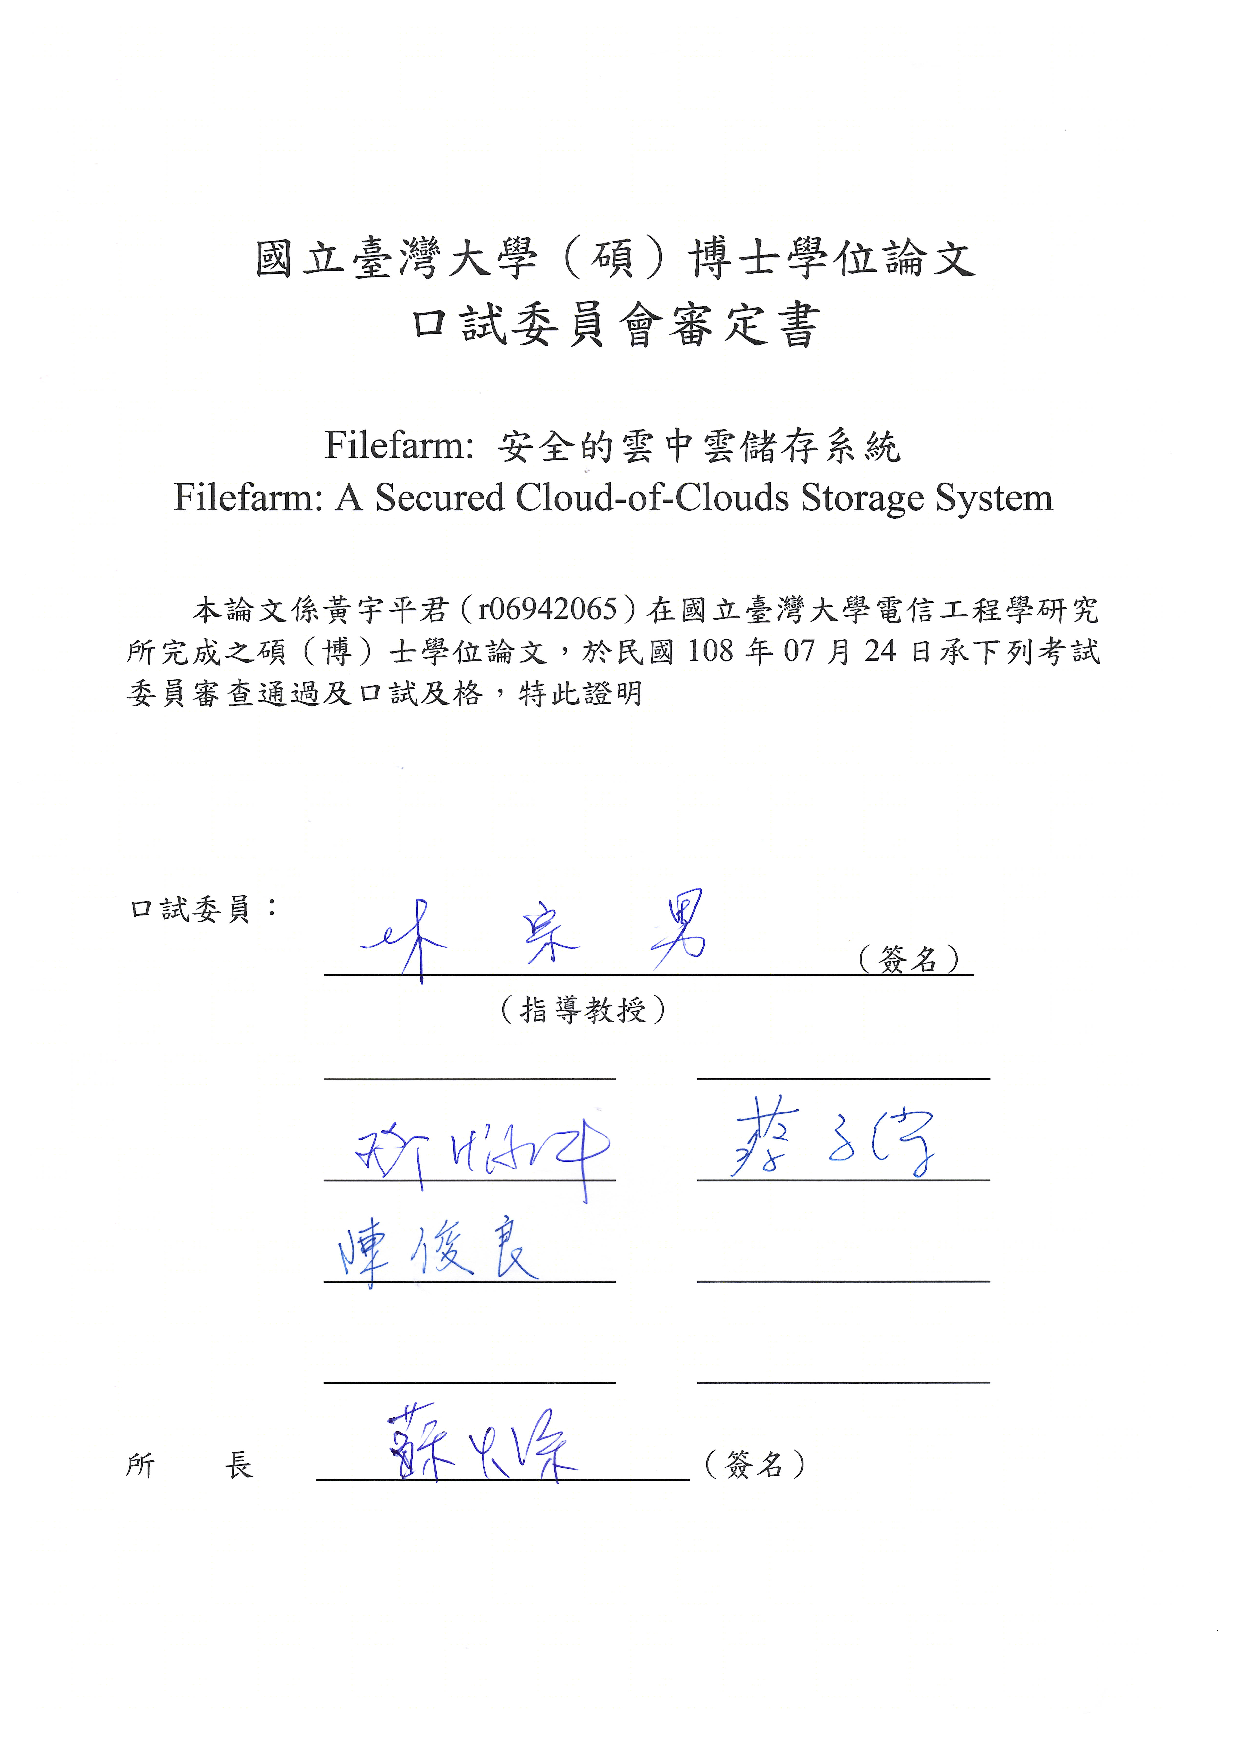
\includepdf[angle=0]{certification.pdf}
\else
  \makecertification
\fi

\begin{acknowledgementszh}
感謝\ldots
\end{acknowledgementszh}

\begin{acknowledgementsen}
I'm glad to thank\ldots 
\end{acknowledgementsen}

\begin{abstractzh}
  在這篇論文中,我們描述 FileFarm: 一個建構於現有雲端儲存服務之上,為防止機密資料外洩、提升可靠性並去除對單一雲端依賴而設計的雲中雲儲存系統。 為了解決既有雲中雲設計因集中式資料庫而造成的一致性和負載平衡問題,FileFarm 採取端對端(P2P)的解決方案。在FileFarm中,每個雲端服務皆為可獨立運作的單元,對客戶端提供相同的服務。這些被稱為\textit{Farmer}的單元相互合作,共同組成一個端對端儲存網路。FileFarm可容忍同時發生於至多$K-1$個Farmer上的錯誤,其中$K$為一個可調整的系統參數。當任何Farmer發生問題而無法提供服務時,FileFarm系統會自動開啟一個修補機制,將資料備份到剩餘存活的Farmer上,確保每個資料區塊都在網路中被儲存了至少$K$份。為了在端對端網路中有效率地尋找資源,FileFarm實作了\textit{Kademlia}分散式雜湊表協定\cite{maymounkov2002kademlia}。 FileFarm 從Kademlia 中繼承了許多重要的特性,包含: (1) 備份數維護、 (2) 高效率搜尋、 (3) 負載平衡的設計。除此之外,作為一個企業級儲存系統,FileFarm還需滿足以下四項條件:(1) 資料機密性 (2) 權限管理 (3) 成本效益 (4) 可存取性。 為此,FileFarm以此四個條件為面向分別設計對應的機制: (1) 加密與資訊分散演算法 (2) 分散式認證 (3) 儲存空間釋放與下載次序差異化 (4) 公有雲ID指定規則。我們基於系統所提供的特性將FileFarm與相關文獻進行比較,同時我們實作了一個系統原型並利用此原型進行一系列實驗以驗證我們聲稱的特性。此系統原型同時也是我們所提出的結構化端對端資料儲存解決方案之產品原型。

\bigbreak
\noindent \textbf{關鍵字:}{\, \makeatletter \@keywordszh \makeatother}
\end{abstractzh}

\begin{abstracten}
  In this thesis, we describe FileFarm: a secured storage overlay that leverages existing cloud services to form a cloud-of-clouds storage system with better robustness, no single-point-of-failure and minimal data leakage concerns. To resolve the consistency and load-balancing issues caused by a centralized database design in conventional cloud-of-clouds work, FileFarm adopts a P2P strategy, in which each cloud operates as an independent node providing identical service for clients. The storage nodes, called \textit{farmers}, cooperate with each other to form a peer-to-peer network, which tolerates concurrent failures occurring at any $K-1$ farmers, where $K$ is a configurable system-wise parameter. In case of failure occurring at any farmer, a storage repair procedure will be triggered automatically, which backs up data to surviving farmers and maintains at least $K$ copies of each piece of data. To lookup resources efficiently in a P2P network, FileFarm implements \textit{Kademlia} DHT(Distributed Hash Table) protocol\cite{maymounkov2002kademlia}. Several desired properties of FileFarm are inherited from Kademlia: (1) redundancy maintenance, (2) efficient search and (3) load-balancing design. However, in order to serve as an enterprise-level storage, 4 further properties are required: (1) data confidentiality, (2) access management, (3) cost-efficiency, (4) retrievability. FileFarm meets these requirements by designing corresponding mechanisms, which collectively  make FileFarm a robust, secure and cost-efficient storage solution: (1) Encryption and Information Dispersal Algorithm, (2) Decentralized Authentication, (3) Storage Release and Prioritized Download, (4)Public Farmer ID Assignment. We compare FileFarm with related implementations in various aspects of properties. We also implement a proof-of-concept and perform a series of experiments on it to verify our claims.  The proof-of-concept not only confirms our claims but also serves as a product prototype of our structured P2P file storage solution.

\bigbreak
\noindent \textbf{Keywords:}{\, \makeatletter \@keywordsen \makeatother}
\end{abstracten}


\tableofcontents
\listoffigures
\listoftables

\mainmatter

\chapter{Introduction}
\label{c:intro}

% rise and prominence of cloud storage
\section{Rise and Prominence of Cloud Storage}
\label{s:riseandprominenceofcloudstorage}
Over the past few years, cloud storage has experienced a metamorphosis from a trendy term to a mature technology and successful business. Due to its high reliability, low cost and minimum management overhead, more and more individual users and enterprises have chosen cloud storage as their major storage solution. According to a recent survey from Enterprise Storage Forum\cite{storagetrends2018}, 68\% of the surveyed enterprises includes cloud in their current storage infrastructure and 35\% of them store their company's primary storage data on cloud storage services. Clearly, high cost of storage hardware has lead businesses to outsource the headaches of in-house storage, and cloud storage turns out to be the best alternative.

% concerns of single cloud solution
\section{Concerns of Single Cloud Solution}
\label{s:concernsofsinglecloudsolution}
While cloud has rapidly become the dominant adoption among all kind of storage choices, another aspect of concerns arises. According to a recent market survey done by DataCore\cite{datacore2017survey}, security (57\%), sensitive data (56\%) and regulatory requirements (41\%) were the 3 major concerns that blocks enterprises from migrating to a public cloud. With data outsourced to a third-party cloud provider, privacy settings are beyond the control of the enterprise. In this situation, sensitive data such as banking information or patient's medical records are exposed to the risks of been viewed or mishandled by malicious insiders in the single cloud. In addition, the "single cloud" solution also suffers from some potential risks such as service availability failure or vendor lock-in problem. For example, table \ref{table:cloudstoragecost} shows the major pricing schema of 3 popular cloud storage providers. Besides the monthly per-GB storage fee, consumers also need to pay an non-negligible fee for their per-GB download traffic. As a consequence, with a large amount of data stored on a single cloud, consumers become dependent (i.e. "locked-in") on this vendor's services and are unable to switch to a different vendor - due to the high switching costs.

\begin{table}[hbt]
\centering
  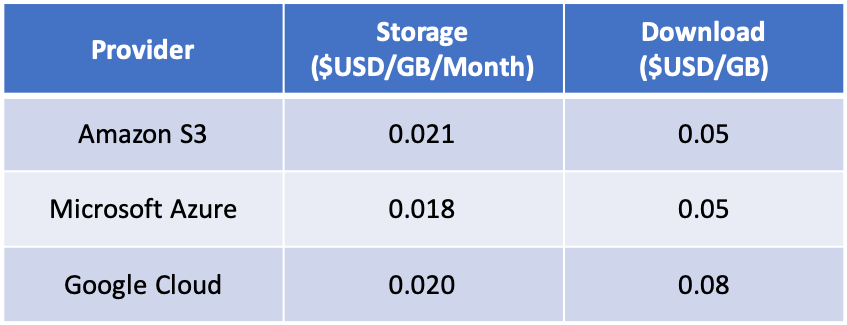
\includegraphics[width=13cm]{tables/table_cloud_storage_cost.png}
  \caption{Major pricing scheme of 3 popular cloud storage providers}
  \label{table:cloudstoragecost}
\end{table}

% FileFarm overview
\section{FileFarm Overview}
\label{s:filefarmoverview}
This paper focuses on resolving the problems caused by dependence on a single storage provider. To be specific, we propose FileFarm, a cloud-of-clouds storage solution that leverages reliability of public cloud storage services while keeping needs from following aspects:

\begin{enumerate}
    \item Preservation of data security and privacy
    \item No reliance on any single cloud
    \item On-demand flexibility of switching between clouds
    \item Cost efficiency
\end{enumerate}

In FileFarm, storage nodes named "$farmers$" coordinate with each other to constitute a peer-to-peer storage network, in a sense that service availability has no dependence on any single farmer. Thus, there is no single-point-of-failure in the FileFarm storage network. With respect to the working flow, each farmer in FileFarm is linked with exactly 1 storage provider (either a public cloud or a private data server) and runs an independent server that provides storage services in terms of GET, PUT, DELETE APIs. To access FileFarm, an authenticated client establishes a stateless connection with any 1 farmer. Since the services provided by farmers are identical, a client can upload a data chunk to FileFarm through one farmer and download it later through another. FileFarm takes care of redundancy automatically, with redundant copies of data distributed over the network. When a farmer encounters service failure, an additional copy of each data chunk it stored will be stored by another farmer automatically. In case of a new farmer joining the network, storage load on each farmer will be balanced automatically.

\chapter{Related Works}
\label{c:related_works}

This chapter surveys previous works in the domain of cloud-of-clouds and distinguishes FileFarm from these works. To preserve data confidentiality and avoid service availability failure caused by dependence on a single cloud, research related to cloud-of-clouds, or in other words, "multi-clouds" or "interclouds", has emerged and received increasing attention. Generally speaking, the main goal of cloud-of-clouds research is to seek a reliable and cost-efficient way to disperse data across multiple cloud providers and avoid dependence or data leakage on any of them. Indeed, an adequate cloud-of-clouds design needs to take a wide variety of aspects into consideration. To make a clear comparison among these works, we arrange this chapter into several sections, each discussing an important aspect to be considered and the corresponding mechanisms employed by each work. In the end of each section, we demonstrate the approach adopted by FileFarm and explain the differences between FileFarm and other cloud-of-clouds works.

\begin{table}[!b]
\centering
  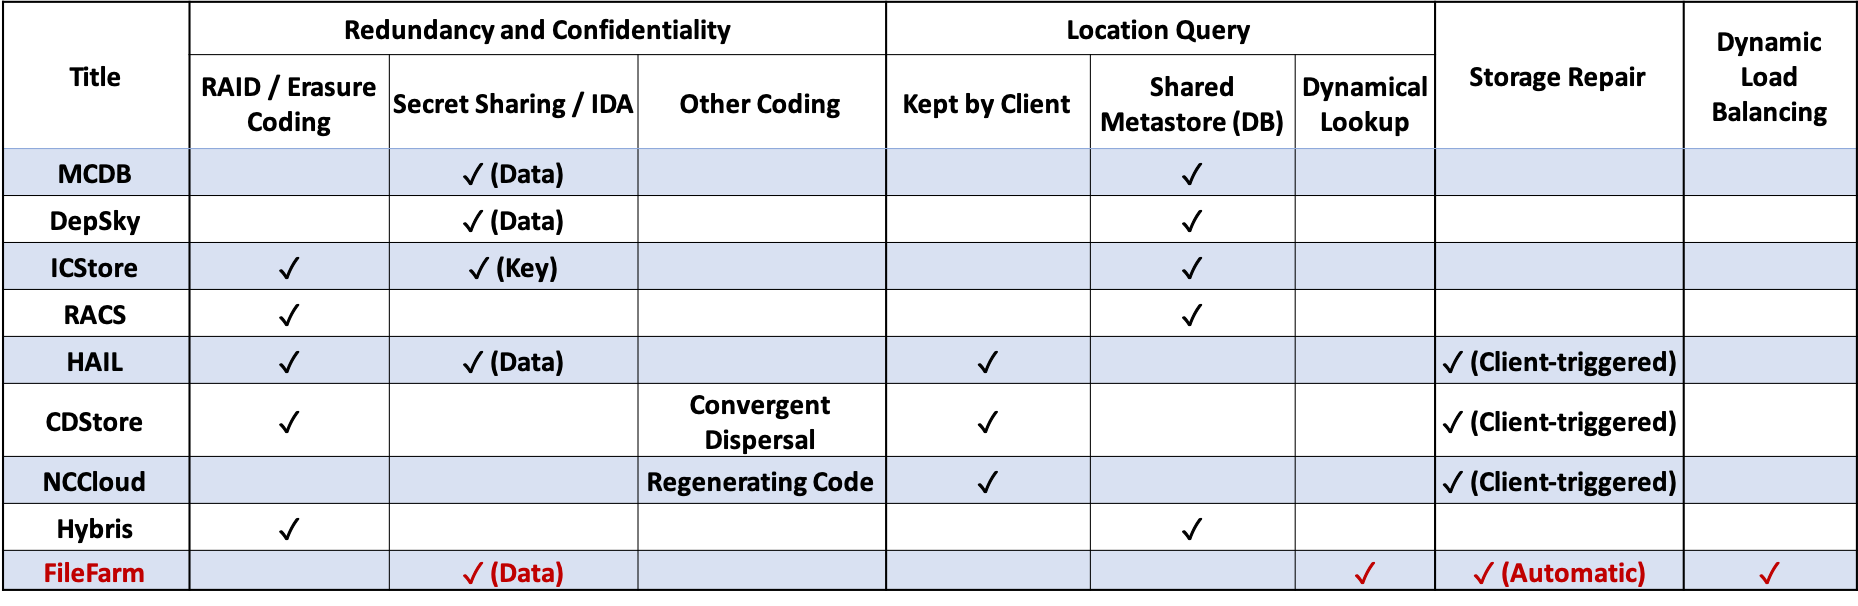
\includegraphics[width=15cm]{tables/table_property_comparison.png}
  \caption{Comparison of properties provided by related cloud-of-clouds designs}
  \label{table:propertycomparison}
\end{table}

% redundancy and confidentiality
\section{Redundancy and Confidentiality}
\label{ss:cocredundancyandconfidentiality}

To avoid dependence of data retrievability on a single cloud, redundancy mechanisms need to be introduced into design of cloud-of-cloud systems. To provide redundancy, RACS\cite{abu2010racs} and HAIL\cite{bowers2009hail} claim their approaches as RAID-like techniques used by disks and file systems, but at the cloud service level. By striping data across multiple providers, RAID-like approach helps customers to avoid vendor lock-in, reduce the cost of switching providers, and better tolerate provider outages or failures. The same benefits can also be provided by erasure coding, which is implemented in ICStore\cite{cachin2010dependable}, CDStore\cite{li2015cdstore} and Hybris\cite{dobre2014hybris}. In fact, RAID-like and erasure coding approaches do not differ too much from each other in the cloud context, considering the fact that cloud storage services usually provide simple key/value store APIs but not a fully functional disk; thus the RAID-like approach does not literally works like an array of pre-allocated storage spaces. Instead, it is more reasonable to view it as an array of redundant data chunks stored on different clouds, which is in the same sense as the erasure coding mechanism.

Besides erasure coding, secret sharing mechanisms such as Shamir's Secret Sharing\cite{shamir1979share} and Information Dispersal Algorithm\cite{rabin1989efficient} also provides redundancy as their side benefit. These mechanisms splits a piece of data into several, say $n$, encrypted chunks, with the assurance that a certain number $m <= n$ of these encrypted chunks are sufficient for recovering the original data. Thus, these secret sharing mechanisms provide advantages in both redundancy and confidentiality. The mechanisms are employed by MCDB\cite{alzain2011mcdb}, DepSky\cite{bessani2013depsky}, ICStore\cite{cachin2010dependable}, HAIL\cite{bowers2009hail}, and also FileFarm.

There are still some other coding mechanisms designed` to provide redundancy and confidentiality for cloud-of-cloud storage. For instance, CDStore\cite{li2015cdstore} is built on an augmented secret sharing scheme called convergent dispersal, which provides benefits of deduplication, storage savings and robustness against side-channel attacks. NCCloud\cite{hu2012nccloud} use functional minimum storage regenerating code (F-MSR) to achieve cost-effective repair for a permanent single-cloud failure.

% location query
\section{Location Query}
\label{ss:coclocationquery}

In a cloud-of-clouds storage system, each data chunk is distributed over some(but not all) of the clouds. To store files and retrieve them back successfully and efficiently, the system must define a way for clients to query which clouds their files are stored on, which we call \textit{location query}. Systems like HAIL\cite{bowers2009hail}, CDStore\cite{li2015cdstore}, NCCloud\cite{hu2012nccloud} focus more on retrievability and algorithms of dispersal while emphasizing less on this part. From these works, we can only inferred that location information is either kept by clients or managed by other layers that are integrated with these systems.

Systems like MCDB\cite{alzain2011mcdb}, DepSky\cite{bessani2013depsky}, ICStore\cite{cachin2010dependable}, RACS\cite{abu2010racs}, Hybris\cite{dobre2014hybris} addresses another solution to location query. In these systems, location information is stored on a shared \textit{metastore}, which is implemented in form of database or simple key/value store. By applying the metastore design, clients in these systems can efficiently get acknowledged of the clouds from which they can download data, within one or few database queries. This provides a convenient and strait-forward way for clients to access their data. Besides, since meta information is stored separately from data, the risk of malicious insider threats on clouds can be reduced significantly. For instance, Hybris\cite{dobre2014hybris} advocates a hybrid cloud structure in which meta data are stored on trusted premises of private servers while encrypted data chunks are stored on untrusted public clouds. With such trust-boundrary design, Hybris leverages strong consistency of meta data stored off-clouds to mask the weak consistency of data stored in clouds.

Nevertheless, there are several issues related to such metastore designs. First, since the mapping between files and clouds is saved as static database records, the records will become out-of-date if some clouds encounter service outage, which has a direct impact on retrievability of files. Second, the static approach has a lack of mechanisms for dynamical replication of shard when encountering permanent single-cloud failures. As a result, the systems have low tolerance for less-reliable providers or successive change of clouds over a long period of time. Third, considering the cases of new clouds joining the system, it takes high cost to re-distribute the data over all clouds; thus these systems would suffer from load-balancing issues and high vendor-switching cost inevitably. Last but not the least, the metastore is regarded as a logically-centralized layer. In spite of the fact that this layer might be implemented with Byzantine Fault Tolerance algorithms or distributed synchronization tools (e.g. Apache ZooKeeper\cite{zookeeper}), the system cannot work without this layer, while any fault occurring to this layer will pose an direct impact on the whole system.

To solve the problems caused by a logically-centralized metastore layer, FileFarm adopts a distributed approach for location query. In FileFarm, clouds coordinate with each other to form a peer-to-peer storage network, while data chunks can be located with an efficient and dynamical lookup procedure defined by Kademlia\cite{maymounkov2002kademlia} DHT protocol. Without a centralized layer storing static information, location query mechanism in FileFarm does not suffer from out-of-date issue and is robust to churn of clouds and network changes in terms of topology or scale. This is the fundamental difference between FileFarm and traditional approaches for cloud-of-clouds. Based on this architectural difference, FileFarm is able to carry out more features that can not be handled well by centralized or hierarchical solutions, such as automatic storage repair, load-balancing, and better degree of fault tolerance.

% storage repair
\section{Storage Repair}
\label{ss:cocstoragerepair}

An important property of cloud-of-clouds systems is disaster recovery. To be specific, when a cloud encounters service failure, the redundancy of each data chunk it used to stored is reduced by a certain factor. To maintain consistent level of redundancy, a \textit{storage repair} mechanism needs to be included in the cloud-of-clouds system design. For an erasure coding based system, an instinctive approach toward storage repair is to let clients download sufficient chunks of data back, reconstruct the lost chunk, and then re-distribute it to other clouds. This is the exact approach implemented by HAIL\cite{bowers2009hail} and CDStore\cite{li2015cdstore}. In fact, this is a general procedure for storage repair that can be employed to all coding-based redundancy schemes, while not explicitly described by some of the related works. Besides the general procedure described above, some systems meet requirements of storage repair with different coding mechanism, seeking to reduce the repair traffic. For instance, NCCloud\cite{hu2012nccloud} uses network coding based scheme to maintain the same data redundancy level as erasure codes, but uses less repair traffic.

While the download-and-redistribute approach managed to repair storage failure and preserve consistent level of redundancy, it is considered to be unfeasible for one primary reason: the mechanism requires \textit{clients} to detect and trigger the entire storage repair procedure manually, which violates the design pattern of cloud services where service reliability should be maintained by the service provider internally and should not rely on any action of clients.

To address this issue, FileFarm adopts a different approach toward storage repair by leveraging its distributed nature. In FileFarm, each stored chunk of data is "re-published" by exactly one storage node in a period of time. As public clouds are considered to be robust, the period can be set long, say, one month. When a cloud encounters service failure, the republish mechanism will repair redundancy automatically within the following one period, without any involvement of other parties required. The same mechanism also offers benefits of load-balancing when new clouds join the network, which will be explained in \ref{ss:storagerelease}. The automatic load-balancing and storage repair properties also make a clear distinction of FileFarm from other cloud-of-clouds works.

% MCDB: use secret-sharing algorithm to avoid the risk of malicious insiders in the cloud and to avoid the failing of cloud services. 


% DepSky: using an efficient set of Byzantine quorum system protocols, cryptography, secret sharing, erasure codes and the diversity that comes from using several clouds.


% ICStore: ICStore client consists of three core layers that target different dependability aspects: i) confidentiality, ii) integrity and iii) reliability and consistency (RC). This layered approach allows individual layers to be switched “on” and “off” to provide different levels of dependability that are to be matched with client’s goals, also with performance and possibly even monetary constraints in mind. In addition, each layer can be individually tuned, as we detail in the following.


% RACS: applying RAID-like techniques used by disks and file systems, but at the cloud storage level. We argue that striping user data across multiple providers can allow customers to avoid vendor lock-in, reduce the cost of switching providers, and better tolerate provider outages or failures


% HAIL: manages file integrity and availability across a collection of servers or independent storage services. It distributes data blocks over servers with information dispersal algorithm and makes use of PORs as building blocks by which storage resources can be tested and reallocated when failures are detected.


% CDStore: builds on an augmented secret sharing scheme called convergent dispersal, which supports deduplication by using deterministic content-derived hashes as inputs to secret sharing. achieve both bandwidth and storage savings and be robust against side-channel attacks.

% NCCloud: use regenerating codes to achieve cost-effective repair for a permanent single-cloud failure. propose an implementable design for the functional minimum- storage regenerating code (F-MSR), which maintains the same data redundancy level and same storage require- ment as in traditional erasure codes (e.g., RAID-6), but uses less repair traffic.


% Hybris: Hybris disperses data (using replication or erasure coding) across multiple untrusted and possibly inconsistent public clouds, while it replicates metadata within trusted premises of a private cloud. Hybris tolerates up to f arbitrary public cloud faults and is very efficient: in the common-case (with replicated variant of Hybris), writes accesses only f + 1 clouds, while a reads accesses a single, “closest” cloud. In a sense, Hybris is the first multi-cloud storage protocol that makes it possible to tolerate potentially malicious clouds at the price of tolerating simple cloud outages. To complement this, Hybris offers strong consistency as it leverages strong consistency of metadata stored offclouds to mask the weak consistency of data stored in clouds.


\chapter{Background}
\label{c:background}

In this chapter, we review important properties of several technologies or terms that are used in FileFarm.

% Cloud Computing
\section{Cloud Computing}
\label{s:cloudcomputing}

Cloud computing is a model describing the relationship between computing resources, service providers and consumers over network connections. In this model, service provider makes effort to offer consumers a convenient, reliable and on-demand way of accessing computing resources. The provider's computing resources are normally pooled to serve multiple consumers using a multi-tenant way with different physical and virtual resources dynamically assigned and reassigned according to consumer's demand. From consumer's point of view, the capabilities available often appear to be unlimited and can be elastically provisioned and released in any amount as long as they need. Furthermore, the resource usage can usually be measured with certain metrics (e.g., storage, processing, bandwidth and active user accounts) and be reported to both provider and consumers transparently. Based on a signed contract, provider then charges consumers in regular basis according to resource usage.\cite{mell2011nist}

With cloud computing technology, enterprises obtain an easy way toward computing outsourcing, in a sense that they no longer need to commit a large amount of capital on hardware and software to build their own IT infrastructure before product launch. Instead, they can rapidly allocate just-enough computing power and storage space as they need with minimal management overhead. They can also elastically expand or reduce the amount of allocated resources based on changes of business scale. Due to the flexibility and reliability, cloud computing has given rise to a paradigm shift in how computing services are deployed and delivered.\cite{6123700}

% Cloud Storage Service
\section{Cloud Storage Service}
\label{s:cloudstorageservice}

Among all types of cloud computing services, storage is nearly the most fundamental one that many others are built upon. To offer a reliable, widely-available cloud storage service, providers build infrastructure and data centers spanning all over the world. Besides hardware deployment, providers also develop software to take care of aspects such as access management, resource routing, replication schema, error correction code, load-balancing... All efforts done by providers contribute to a single purpose: to provide consumer with a robust, easy-to-access online disk space. From consumer's point of view, the storage service seems much more simpler. To access the storage service, consumers connect to provider's server using a pre-defined API. The allowed API operations should at least include POST, GET, DELETE, by which consumers can upload, download and remove data, respectively.

Cloud storage service is a mature technology and business that changes the way data are stored and accessed. Among all existing cloud storage services, Amazon AWS S3\cite{awss3}, Google Cloud Storage\cite{googlecloudstorage}, Microsoft Azure\cite{msazurestorage} are 3 successful instances. Depending on usage size, access rate and service-level agreement, a storage provider may provide various storage service products. The pricing schema of cloud storage services usually involves 2 major usage factors: (1) \textit{static storage} (2) \textit{data transfer}. The former one is the fee of storing data statically, charged in per GB/month basis, whereas the latter one charges consumers every GB of data downloaded from the cloud (upload traffics are usually for free). The 2 factors collectively account for the primary part of storage fee.

Cloud storage services have successfully relieve individual or enterprise consumers from affording the high cost of maintaining their own storage systems. Due to the economies of scale, cost of cloud storage solution is usually much lower than that of building a storage infrastructure with same level of reliability on consumers' own. Thus, cloud storage has gradually dominated the choice of enterprises over other storage options\cite{storagetrends2018}.

% Cloud-of-Clouds
\section{Cloud-of-Clouds}
\label{s:cloudofclouds}

Although cloud computing provides benefits in terms of low cost, elasticity and reliability, ensuring security of data stored on clouds remains an unsolved problem, as consumers often store critical and sensitive data on the services offered by a third-party provider which may be untrusted. To solve this issue, researchers have moved forward to  a new research domain\cite{aizain2012multiclouds}. "Cloud-of-clouds", or "multi-clouds", "interclouds" is an area of research aiming to build a service on multiple clouds and avoid dependence or data leakage on any of them. The term was firstly introduced by Vukolic\cite{vukolic2010byzantine}. Multiple works have been proposed at around the same time\cite{bowers2009hail},\cite{abu2010racs},\cite{cachin2010dependable},\cite{bessani2013depsky}. The research in this area has often been formulated as a Byzantine fault tolerance problem\cite{lamport1982byzantine}, in the sense that any faults occurring to a cloud may lead to misbehavior of it, while the system is designed to tolerate certain level of concurrent cloud failures. Besides, approaches of solving the single-cloud problem often integrate certain means of coding techniques that not only add redundancy to data, but also make sure that a file is not view-able or recoverable from any single cloud. This way, risks of malicious insider or single cloud service failure can be reduced significantly.

% Hybrid Cloud
\section{Hybrid Cloud}
\label{s:hybridcloud}

Hybrid cloud is a specialized branch of cloud-of-clouds research. In the settings of hybrid cloud, part of the enterprises' service is held by their own servers. Integration of both public clouds and private servers contributes to a more rapid and robust service. Such hybrid design is actually a more practical and feasible deployment option for most enterprises. As mentioned above, public clouds bring benefits of reliability, flexibility and cost-efficiency; however, they cannot provide certain benefits of servers in private network, such as security, low-latency and full control over data. With proper design, hybrid cloud systems have the potential of bringing the best of both public clouds and private premises, while minimizing the disadvantages of them. A cloud storage example under this topic is: \textit{Hybris}\cite{dobre2014hybris}.

% Peer-to-Peer Systems
\section{Peer-to-Peer Systems}
\label{s:peertopeersystems}

Peer-to-Peer is a computing or networking architecture in which each participant, called a \textit{node} or a \textit{peer}, shares equal responsibility of maintaining the dedicated service. In a P2P system, peers are equally-privileged and follow the same protocol to negotiate with each other, without a centralized coordinator over them. Instead of aggregating storage and computing power to a single serving machine, each peer in a P2P system contributes part of their resources to the network, and requires the resources they want from other peers in return. A properly-designed P2P system will eventually meet all peers' need. Because of the distributed architecture, P2P model does not suffer from single-point-of-failure problem, which means such systems are generally robust to frequent churning of peers, network topology changes, or failures occurring to part of the network. Besides, since peers serve need for each other without a centralized channel, P2P systems tend to have better throughput and service capability than traditional client-server model. However, since there are no central node in a P2P network, a peer needs to coordinate with other peers on it's own and achieve a consistent state of consensus with others, in terms of routing information, content location, status of other peers, ... This brings extra computational and timing overhead to peer applications. Due to this, P2P protocols are usually more difficult to design then client-server ones, and some P2P systems are suffering from efficiency and scalability issues. Despite of the difficulty, P2P systems had still found its popularity in many application domains, with content sharing being the origin of the whole concept and the most successful one so far. \textit{Napster}\cite{napster}, \textit{BitTorrent}\cite{bittorrent}, \textit{eMule}\cite{emule}, \textit{aMule}\cite{amule} are some successful P2P content sharing applications.

% Distributed Hash Table
\section{Distributed Hash Table}
\label{s:distributedhashtable}

How to search for data over a fully-distributed network has always been a research topic drawing high attention. Of all kind of means proposed, distributed hash table (DHT) is the most popular category due to its high efficiency. Generally speaking, DHT is a content-addressed approach in which each piece of data is assigned with a \textit{key} defined as its hash value. The piece of data is then stored in the distributed network according to its \textit{key}. Thus, the locations where a given piece of data should be stored are defined by its content. This introduces deduplication feature for such systems since same content will always be stored on same set of nodes. Besides, the dispersal and randomness properties of hash function also enable DHT-based systems to be designed in a load-balancing way. In P2P applications, DHTs are often implemented as an overlay or infrastructure that more complex services can be built upon. Such applications then inherit the desired features of their underlying DHTs. A DHT protocol also defines how to lookup and retrieve data from the network. Efficiency of the lookup process has a direct impact on performance and usability of systems based on the DHT. Most of the widely-used DHTs have logarithm-time guarantee on worst-case lookup length. Chord\cite{stoica2001chord}, Kademlia\cite{maymounkov2002kademlia}, Pastry\cite{rowstron2001pastry}, Tapestry\cite{zhao2004tapestry} are some well-known DHT protocols, to name a few.

% Kademlia
\section{Kademlia}
\label{s:kademlia}
Kademlia\cite{maymounkov2002kademlia} is a popular structured DHT protocol applied on a number of modern P2P applications including BitTorrent\cite{bittorrent}, Ethereum\cite{ethereum}, IPFS\cite{ipfs} and Storij\cite{storij}, ... The wide adoption of Kademlia can be attributed to several desired properties it provides. We categorize these properties into 3 aspects: \textit{load balancing}, \textit{efficient search} and \textit{redundancy maintenance}.

\subsection{Load Balancing}
\label{ss:loadbalancing}
In a Kademlia network, storage load of composing nodes are roughly balanced. This property is assured by the underlying ID assignment and content-addressable designs. In Kademlia, each node is assigned with a randomly-generated 160-bit ID when it starts up. Besides, each data chunk to be stored in the network is identified by its SHA-1 hash value (aka. \textit{key}), which is also 160 bit in length. Since node IDs and keys share exactly the same format, they are also able to share the same \textit{distance metric}. Given 2 identifiers (node ID or key), $x$ and $y$, the distance between them is defined as their bit-wise exclusive or (XOR) interpreted as an integer, $\delta(x,y)=x \oplus y$. With distance metric defined, Kademlia further regulates that each piece of data should be stored at the \textit{$K$ nodes with ID closest to the its key}, where $K$ is a system-wise redundancy parameter. Due to the randomness of node IDs and keys, data pieces are uniformly distributed over the storage nodes, with each node's load expected to be balanced.

\subsection{Efficient Search}
\label{ss:efficientsearch}

Kademlia provides an efficient way to search for a piece of data in a P2P network given its \textit{key}. Like many other DHT alternatives, it takes no more than $\lceil log(n) \rceil + c$ iterated queries to lookup any target in a Kademlia network. In this subsection, we explain the lookup mechanisms of Kademlia in detail.

As described in \ref{ss:loadbalancing}, a piece of data should be stored on the $K$ nodes with ID closest to the its key. These $K$ nodes are uniquely defined by the XOR distance metric, and can be found by lookup procedures specified in Kademlia protocol. To know how these procedures work, we first take a look at how routing information is kept on each node. Kademlia's ID space can be represented as a binary tree (also called \textit{trie}) of height 160, with each ID representing a leaf node in the trie. Figure \ref{fig:buckettrie} shows an example of the trie in a small Kademlia network where ID length $d = 4$. The leaves of this trie represent all possible node IDs in this network. Given an ID $x$, the trie can be partitioned into $d$ subtrees as follows:

\begin{center}
  $D_{i}(x) = {y: \delta(x,y) \in [2^{i-1}, 2^{i}]}, i = 1, 2, ..., d$
\end{center}

Notice that IDs in each subtree share the same prefix, where the last bit of the prefix indicates the most significant difference bit between $x$ and IDs in the corresponding subtree, which determines the distance from these IDs to $x$. Thus, the longer the prefix is, the closer the IDs are to $x$. For instance, IDs in $D_{2}(x)$ share prefix $101$, which indicates that all IDs in $D_{2}(x)$ share the same first 2 bits with $x$ while their third bit is different from $x$. Thus, distance between x and IDs in $D_{2}(x)$ ranges from $2^{1}$ to $2^{2}-1$. From this point of view, it is clear that this partition splits the entire ID space into $d$ parts according to the XOR distance metric.

\begin{figure}[hbt]
  \centering
    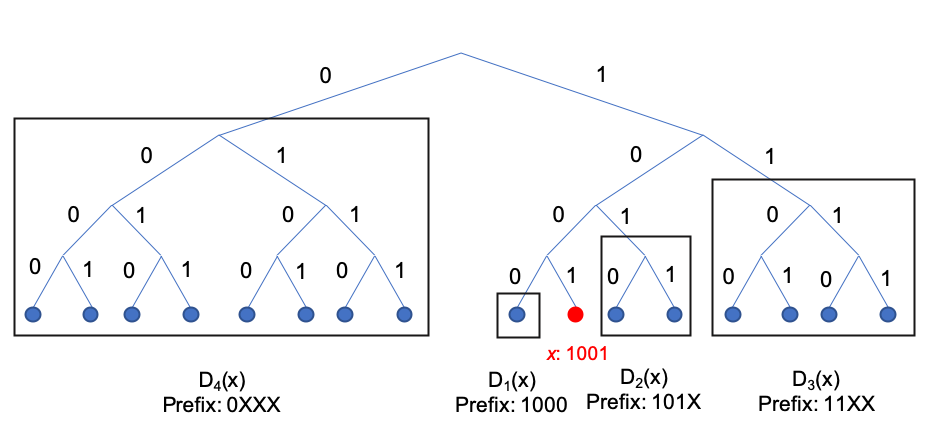
\includegraphics[width=13cm]{figures/bucket_trie.png}
    \caption{An example of Kademlia's Trie with ID length = 4}
    \label{fig:buckettrie}
\end{figure}

In Kademlia, a node with ID $x$ maintains a routing table that keeps at most $K$ records of peers for each subtrees in $D_{1}(x), D_{2}(x), ..., D_{d}(x)$. With this routing table, the node is acknowledged of peers' contact information from a wide range of distance.

Before explaining details of lookup procedures, we define 2 types of RPCs (Remote Procedure Call) used by Kademlia nodes to communicate with each other:
\begin{itemize}
  \item \textit{FIND\_NODE}:
  \begin{itemize}
    \item \textbf{Input}: a 160-bit TARGET\_ID
    \item \textbf{Output}: $K$ triples of \textit{<IP address, UDP port, Node ID>} known by the receiver with Node IDs closest to TARGET\_ID
  \end{itemize}
  \item \textit{FIND\_VALUE}
  \begin{itemize}
    \item \textbf{Input}: a 160-bit TARGET\_KEY
    \item \textbf{Output}: 
    \begin{itemize}
      \item The data chunk with key being TARGET\_KEY; if the receiver does store the data chunk with key being TARGET\_KEY
      \item $K$ triples of \textit{<IP address, UDP port, Node ID>} known by the receiver which are closest to TARGET\_KEY; otherwise
    \end{itemize}
  \end{itemize}
\end{itemize}

\noindent Now we describe the lookup procedures. In Kademlia, there are 2 types of lookup:
\begin{itemize}
  \item \textit{NODE\_LOOKUP}: to find the $K$ nodes in the network with ID closest to a target ID
  \item \textit{VALUE\_LOOKUP}: to find the content corresponding to a target key
\end{itemize}

\noindent \textbf{Algorithm \textit{NODE\_LOOKUP:}}
\begin{itemize}
  \item \textbf{Input}: a 160-bit TARGET\_ID, $K$ triples of \textit{<IP address, UDP port, Node ID>} known by the initializer with Node IDs closest to TARGET\_ID
  \item \textbf{Output}: $K$ triples of \textit{<IP address, UDP port, Node ID>} in the network with Node IDs closest to TARGET\_ID
\end{itemize}
\begin{enumerate}[label=(\roman*)]
  \item The initializer puts the $K$ closest nodes it knows into a lookup-memory
  \item The initializer picks $\alpha$ nodes from the lookup-memory, where $\alpha$ is a system-wide concurrency parameter, such as 3.
  \item The initializer sends parallel, asynchronous FIND\_NODE RPCs to these $\alpha$ nodes and expect to receive $K$ closest node records known by each of them.
  \item When receiving a FIND\_NODE response containing k node candidates, the initializer updates these candidates to the lookup-memory and leaves only $K$ closest ones. Then the initializer picks $\alpha$ un-queried nodes from the lookup-memory and sends FIND\_NODE RPCs to them
  \item If a round of FIND\_NODE fails to return closer nodes than the ones in the lookup-memory, the initializer sends FIND\_NODEs to all un-queried nodes in the lookup-memory
  \item The NODE\_LOOKUP procedure terminates when the initializer receives all responses. Now the $K$ nodes in lookup-memory are the $K$ closest ones to TARGET\_ID over the network and should be returned.
\end{enumerate}

\noindent \textbf{Algorithm \textit{VALUE\_LOOKUP:}}
\begin{itemize}
  \item \textbf{Input}: a 160-bit TARGET\_KEY, $K$ triples of \textit{<IP address, UDP port, Node ID>} known by the initializer with Node IDs closest to TARGET\_KEY
  \item \textbf{Output}:
  \begin{itemize}
    \item The TARGET\_CHUNK with key being TARGET\_KEY; if TARGET\_CHUNK exists in the network
    \item $K$ triples of \textit{<IP address, UDP port, Node ID>} in the network which are closest to TARGET\_KEY; otherwise
  \end{itemize}
\end{itemize}
\begin{enumerate}[label=(\roman*)]
  \item The initializer puts the $K$ closest nodes it knows into a lookup-memory
  \item The initializer picks $\alpha$ nodes from the lookup-memory, where $\alpha$ is a system-wide concurrency parameter, such as 3.
  \item The initializer sends parallel, asynchronous FIND\_VALUE RPCs to these $\alpha$ nodes.
  \item When receiving a FIND\_VALUE response containing TARGET\_CHUNK, the procedure ends by returning TARGET\_CHUNK
  \item When receiving a FIND\_VALUE response containing $K$ node candidates, the initializer updates these candidates to the lookup-memory and leaves only $K$ closest ones. Then the initializer picks $\alpha$ un-queried nodes from the lookup memory and sends FIND\_VALUE RPCs to them
  \item If a round of FIND\_VALUE fails to return closer nodes than the ones in the lookup-memory, the initializer sends FIND\_VALUEs to all un-queried nodes in the lookup-memory
  \item The VALUE\_LOOKUP procedure terminates when the initializer receives all responses. In this case, the initializer fails to find TARGET\_CHUNK, and the $K$ nodes in the lookup memory closest to TARGET\_KEY should be returned.
\end{enumerate}

Now we want to discuss the efficiency of NODE\_LOOKUP and VALUE\_LOOKUP procedures. According to the sketch of proof in \cite{maymounkov2002kademlia}, NODE\_LOOKUP in a Kademlia network will finish in $\lceil log(n) \rceil + c$ steps for some small constant of $c$, where $n$ is network size, i.e., number of nodes in the network. This gives an rough upper bound for NODE\_LOOKUP efficiency.

Different from NODE\_LOOKUP, the VALUE\_LOOKUP procedure finishes immediately when the target value is found. Thus, VALUE\_LOOKUP procedure only needs to reach any one of the $K$ closest nodes instead of finding all of them. According to Cai's analysis\cite{cai2013probabilistic}, it takes no more than $(1+O(1))\frac{log(n)}{H_{K}}$ steps for any node in a Kademlia network to locate any other node, where $H_K = \sum_{i=1}^{K} 1/i$. This upper bound also stands for VALUE\_LOOKUP, considering the fact that VALUE\_LOOKUP for the target key converges along the same path as NODE\_LOOKUP for the closest farmer, due to \textit{unidirectionality} of XOR distance metric: For any given point $x$ and distance $\Delta>0$, there is exactly one point $y$ such that $d(x,y)=\Delta$.

From the analysis above, we know that both NODE\_LOOKUP and VALUE\_LOOKUP procedures are guaranteed to be finished in logarithm steps, while VALUE\_LOOKUP takes a tighter bond with a factor of $H_K = \sum_{i=1}^{K} 1/i$, since only 1 copy of data is required to be found, and we can find it by reaching any of the $K$ storing nodes.

\subsection{Redundancy Maintenance}
\label{ss:redundancymaintenance}
Redundancy maintenance is another desired property provided by Kademlia. When a node churns off from the network, each of the data chunks it used to stored will lose one redundancy copy. Kademlia has a \textit{Efficient Key Republishing} mechanism ensuring that each chunk will always have at least $K$ copies over the storage network.

The \textit{Efficient Key Republishing} mechanism regularly checks if each data chunk is stored on the $K$ closest farmers. If any of the $K$ closest farmers does not store the chunk, a copy will automatically be sent to it. This assurance is provided by the design in which each farmer periodically attempts to \textit{republish} each chunk it stored to the other $K-1$ farmers who should store the same chunk. During the republishing period, if a farmer receives the republishing message of a chunk from other farmer, it assumes the message has also been sent to the other $K-1$ closest farmers and thus it should not republish it again during this period in order to reduce traffic. As long as the republishing interval of farmers are not exactly matched, there will only be exactly 1 republishing message for each chunk in each interval. However, the Efficient Key Republishing mechanism has a considerable overhead. Within a \textit{republishing period}, each chunk induces one NODE\_LOOKUP followed by $K$ republishing messages. Choices of longer republishing period would mitigate the overhead while providing weaker guarantee on retrievability of files.

% Information Dispersal Algorithm
\section{Information Dispersal Algorithm}
\label{s:informationdispersalalgorithm}

An Information Dispersal Algorithm (IDA)\cite{rabin1989efficient} is a computation schema of disperse content of a file into smaller chunks and reconstructing the original file based on some of the chunks, where the dispersal and reconstruction process are computationally efficient. To be more precise, a $(p,q)$ IDA schema breaks a file $F$ into $p + q$ chunks of size $\frac{|F|}{p}$, such that $F$ can be reconstructed from any p chunks but not less. Figure \ref{fig:ida} shows an example of dispersing a file $F$ of size $|F|=16$ bytes with a $(4,2)$ schema. In the figure, each byte is represented as an integer from $[0, 255]$. The first step of IDA is to split the original file into $p=4$ chunks, with each chunk being a row of the matrix representing the entire file. After that, a randomly generated matrix $M$ of size $(p+q)\times p$ is being multiplied with the file matrix and the computation yields a matrix of size $(p+q)\times \frac{|F|}{p}$. Each row in the result matrix is a computed chunk that is supposed to be stored in a place different from others. To reconstruct the original file $F$, one needs to collect $p$ computed chunks and multiply the collected chunks with inverse matrix of concatenation of their corresponding rows in $M$. As long as the corresponding rows in $M$ are linearly independent, the original file can be reconstructed based on these $p$ collected chunks.

Due to its potential traits of security, load-balancing and fault tolerance design, Information Dispersal Algorithm is widely-used in distributed file storage or content sharing applications. Considering a distributed network of computers and workstations, files pre-processed with IDA are certainly hard to be reconstructed by nodes other than the uploader, since only the uploading node has the knowledge of dispersion keys and distribution of chunks in the network. In a distributed application, the stored chunks can be downloaded from different nodes in parallel, this boosts the downloading performance of large files.  Also, the $q$ factor in the IDA schema makes redundancy and tolerance in a fault-prone environment. These are reasons why IDA is suitable for distributed systems.

\begin{figure}[hbt]
\centering
  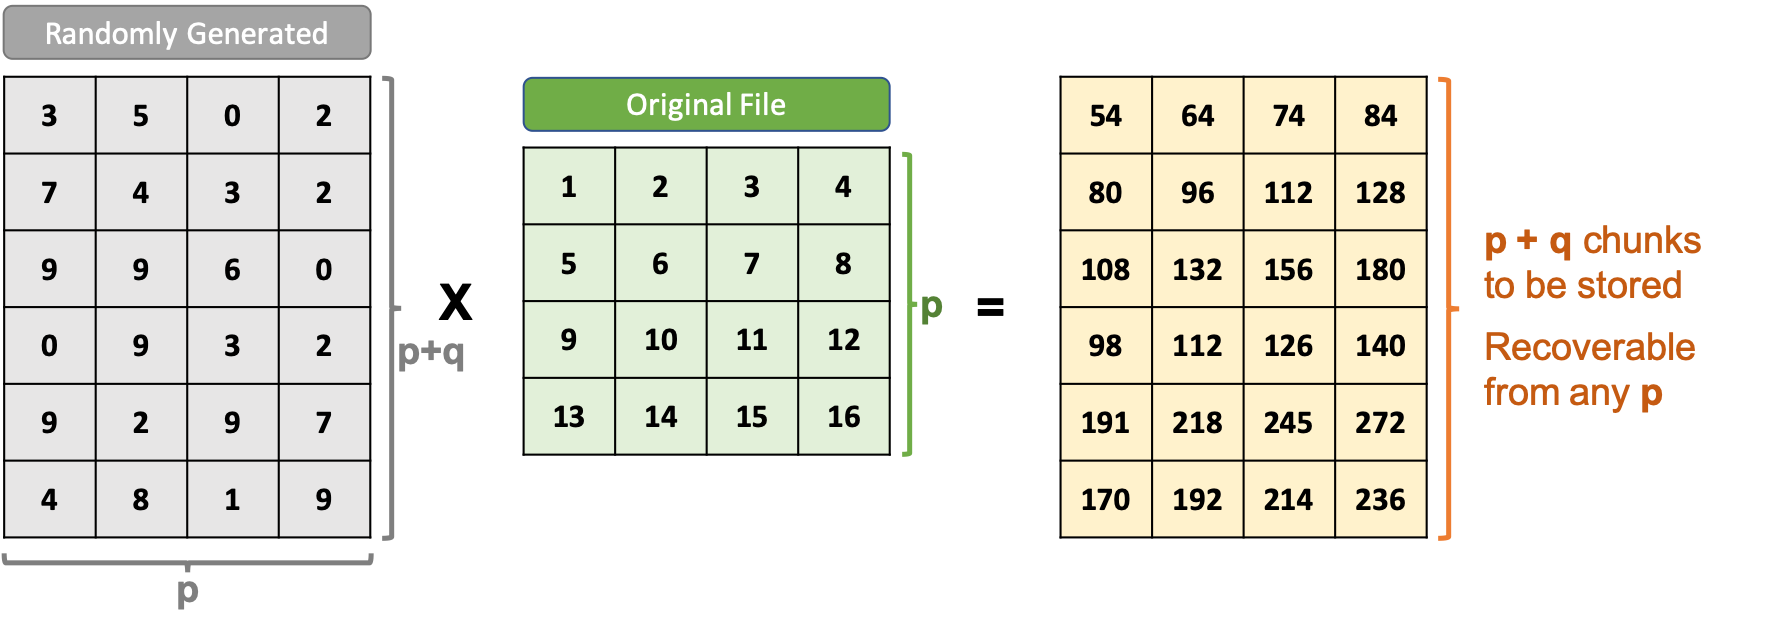
\includegraphics[width=13cm]{figures/ida.png}
  \caption{An example of IDA with schema $(p,q)=(4,2)$}
  \label{fig:ida}
\end{figure}

% Public Key Infrastructure
\section{Public Key Infrastructure}
\label{s:publickeyinfrastructure}

Public key infrastructure (PKI) is an infrastructure that enables entities to securely communicate over an insecure public network via cryptographic techniques of public-key encryption, digital signature and certificate-based authentication. From the perspective of cryptography, PKI is a reliable approach to bind public keys with respective identities. The binding process is facilitated by registration and issuance of digital certificates, which can be demonstrated by Figure \ref{fig:pki}: The whole process involves 3 parties: an entity providing service to users, an certificate authority (CA) and a user. To get a certificate, the entity needs to generate a certificate request (CSR) containing its public key first. It then send the CSR to CA. With all means of verification, CA finally trusts the entity. CA then generates a certificate for the entity, which includes CA's digital signature signed with its private key. The certificate is then sent back to the entity and installed on its server machine. From now on, whenever a user sends a connection request to the entity, it responses with its certificate. The user then verifies this certificate by validating the CA's signature on the certificate. If the verification passes, user will establish a secure connection encrypted by the entity's public key.

PKI is a general term involving policies of issuing, managing, and validating digital certificates. Inside this broad term, X.509\cite{rfc4158} is a majorly adopted standard defining the format of public key certificates, which is widely used in the Internet and is the fundamental technique implemented in TLS/SSL, which is the basis of HTTPS.

\begin{figure}[hbt]
\centering
  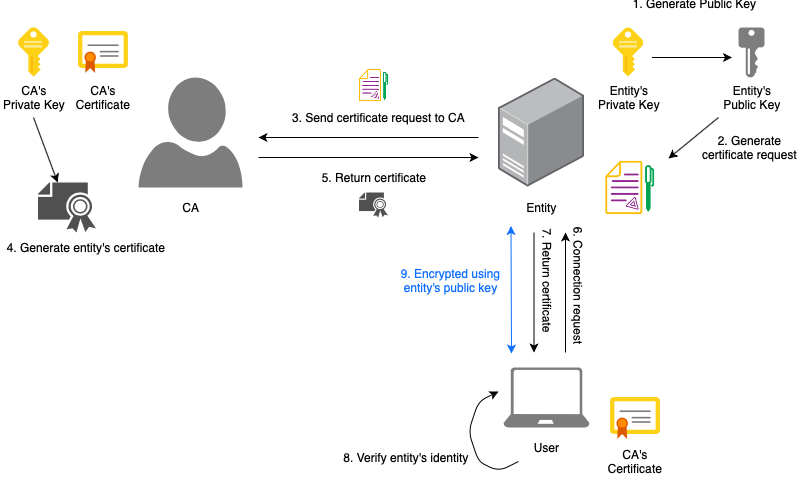
\includegraphics[width=14cm]{figures/pki.png}
  \caption{Procedure of certificate issuance and certificate-based authentication}
  \label{fig:pki}
\end{figure}
\chapter{Methodology}
\label{c:methodology}

In this chapter, we describe the FileFarm system in detail. It starts by presenting the system architecture and roles in the system. Then it shows the model of each building block of FileFarm and the upload / download process flows. Finally it explains each of the desired characteristics FileFarm provides and the mechanisms behind them.

% system architecture
\section{System Architecture}
\label{s:systemarchitecture}

\begin{figure}[hbt]
\centering
  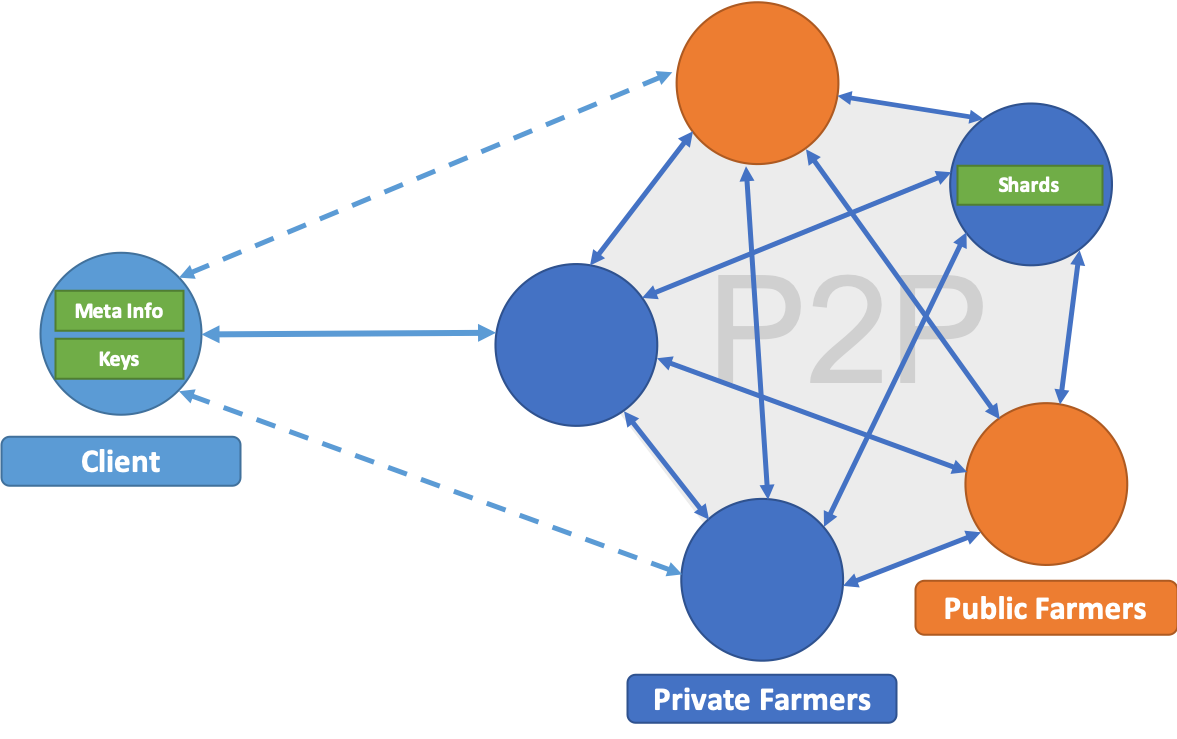
\includegraphics[width=15cm]{figures/system_architecture.png}
  \caption{System architecture}
  \label{fig:systemarchitecture}
\end{figure}

\newpage

\noindent The FileFarm system is composed of 2 roles:

\begin{enumerate}
  \item \textit{Client}: User-side application providing user interface, handling upload/download tasks and managing file meta along with hash values and encryption keys for later retrieval.
  \item \textit{Farmer}: Basic component of the FileFarm storage network. A farmer is linked with exactly 1 storage provider (either a public cloud or a private data server) to offer storage service. At the same time, farmers connect to each other to form a P2P network and take care of availability of each stored piece of data. A farmer also provides API for clients to store and retrieve data.
\end{enumerate}

As shown in Figure \ref{fig:systemarchitecture}, The FileFarm cloud-of-clouds is formed by farmers, in a sense that service availability has no dependence on any single farmer or its underlying cloud. Thus, FileFarm system has no single-point-of-failure. All farmers provide the same storage service. Thus, client can establish stateless connection with any farmer for uploading/downloading data.

The basic unit of data in FileFarm network is called \textit{shard}, which is a computed segmentation of file that is saved in the network. A specific amount of distinct shards are required to reconstruct the original file, depending on the \textit{sharding schema}. From client's point of view, a file is split, encrypted and then computed into a number of shards with IDA (more details explained in \ref{s:dataconfidentiality}). Instead of the original file, the shards are what actually uploaded. The encryption keys, hashes, file meta are kept by client itself. This ensures that only the client itself is able to reconstruct its own data.

\newpage

% application models and process flows
\section{Application Models and Process Flows}
\label{s:applicationmodelsandprocessflows}

\begin{figure}[hbt]
\centering
  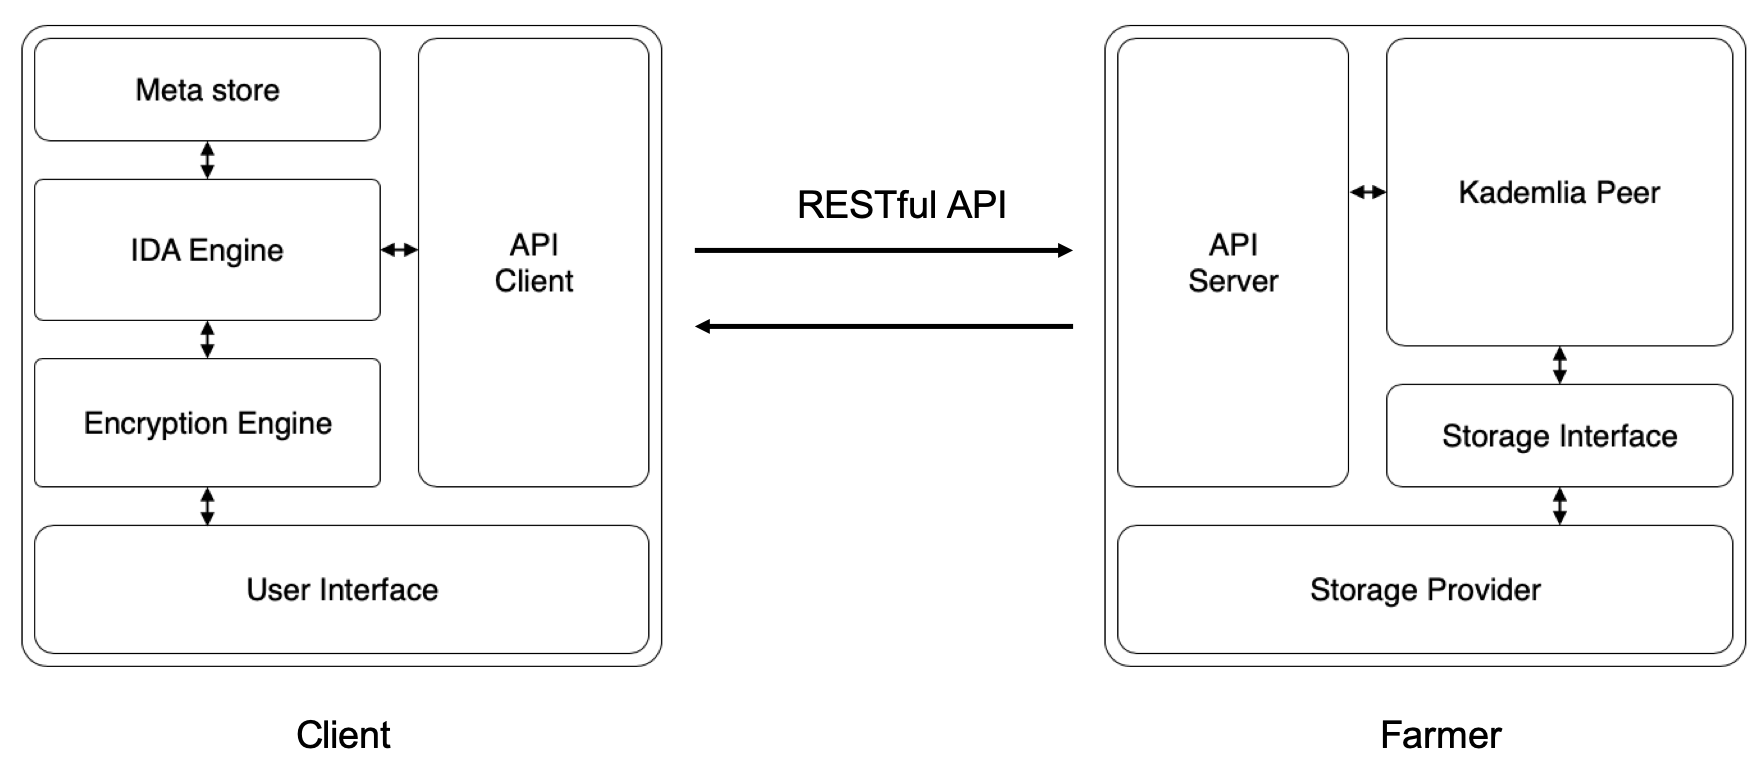
\includegraphics[width=14cm]{figures/application_models.png}
  \caption{Application model of client and farmer}
  \label{fig:applicationmodels}
\end{figure}

Figure \ref{fig:applicationmodels} shows the model of client and farmer applications. Client application has a interface for user to manage their own storage and to upload/download files. When receiving command from user to upload a file, the client application splits the file into slices and pre-process each slice with encryption engine and IDA engine. After pre-process, each slice is transformed into multiple shards, and the encryption keys and hash value of shards are saved in the client's meta store at the same time. The client application then upload each shard to the FileFarm storage network through a randomly-chosen farmer. Farmer application, on the other hand, has a API server module that serves request from client applications. Besides the server module, farmer also has a Kademlia peer module that coordinates with other farmer's corresponding part to synchronize storage status of uploaded shards and provide an efficient way to locate them. In order to apply farmer application on different storage services, FileFarm implements an abstract storage interface layer that provides identical out-bounded API but negotiate with different storage providers according to their API format.

Going with the application model, we present upload / download flow of FileFarm in figure \ref{fig:uploadflow} and figure \ref{fig:downloadflow}, respectively. Some of the processes in these 2 flow diagrams is not clear yet, which will be explained in the following sections.

\newpage

\begin{figure}[hbt]
\centering
  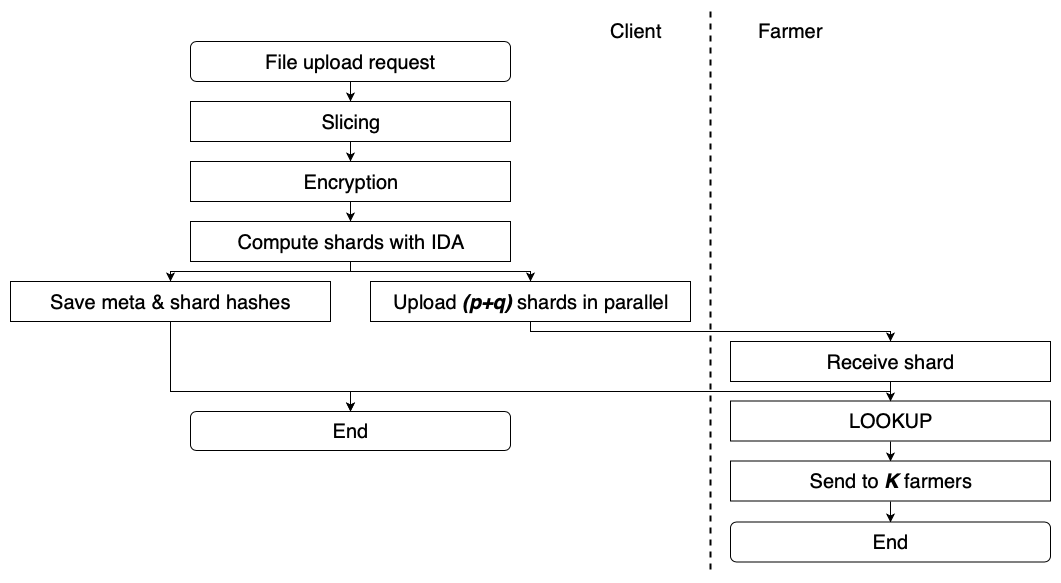
\includegraphics[width=14cm]{figures/upload_flow.png}
  \caption{Upload flow}
  \label{fig:uploadflow}
\end{figure}

\begin{figure}[!b]
\centering
  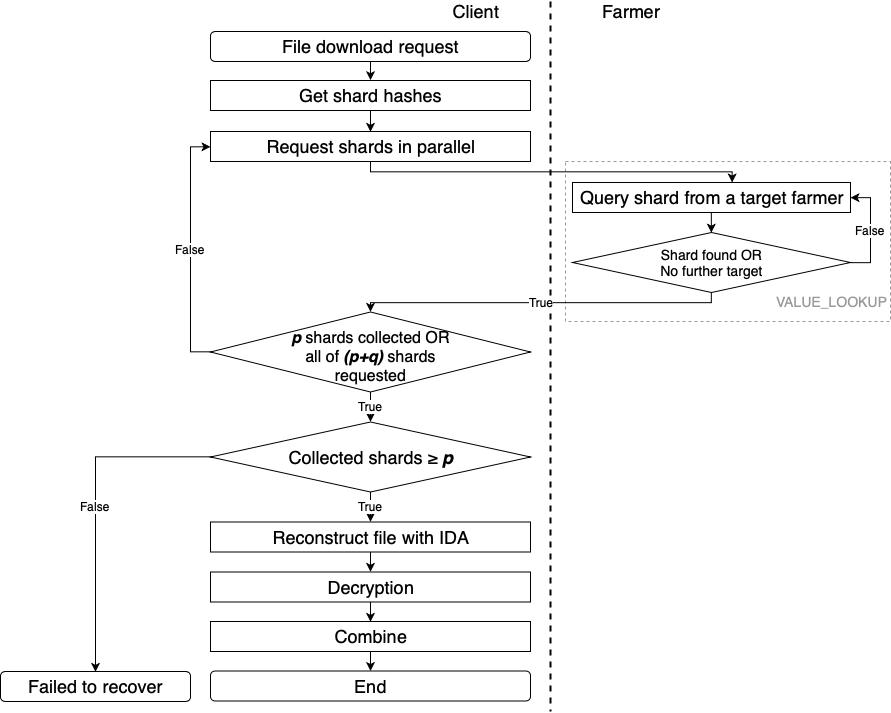
\includegraphics[width=15cm]{figures/download_flow.png}
  \caption{Download flow}
  \label{fig:downloadflow}
\end{figure}

\newpage

% DHT-based approach
\section{DHT-Based Approach}
\label{s:dhtbasedapproach}

To find shards in a P2P network, FileFarm implements Kademlia DHT protocol. As described in \ref{s:kademlia}, Kademlia protocol gives FileFarm benefits in the following aspects:

\begin{enumerate}
  \item \textit{Load balancing}: storage load of each farmer is roughly balanced.
  \item \textit{Efficient search}: lookups in FileFarm needs no more than logarithm steps.
  \item \textit{Redundancy maintenance}: each shard will always be stored on at least $K$ farmers.
\end{enumerate}

Instead of saving location of shards as static records in a centralized database, FileFarm adopts Kademlia's dynamical lookup procedures. Before storing a shard, a farmer uses the NODE\_LOOKUP procedure to determine on which farmers the shard should be stored, and then send parallel storing messages to these farmers. In the case of shard retrieval (download), a farmer performs VALUE\_LOOKUP procedure to find the shard iteratively until it is found. Both NODE\_LOOKUP and VALUE\_LOOKUP procedures are robust to churn of farmers, network topology changes and scaling of network size, which usually can not be handled well in centralized solutions. Besides, since given shard, the $K$ farmers to store it are uniquely defined and the results of NODE\_LOOKUP and VALUE\_LOOKUP procedures have no dependence on originating node, a client can request any farmer to upload or download the shard, which will eventually be stored on the same set of farmers. This allows a parallel and fault-tolerant design in which clients can upload /download different shards from different farmers simultaneously and do not rely on a specific farmer to perform these tasks.

\newpage

% Beyond Kademlia
\section{Beyond Kademlia}
\label{s:beyondkademlia}

From \ref{s:dhtbasedapproach}, we acknowledged that FileFarm inherits a number of benefits from Kademlia. However, Kademlia was originally invented for content-sharing applications but not storage systems. To claim FileFarm as an enterprise storage, we also need to consider following requirements that cannot be provided by Kademlia:

\begin{enumerate}
  \item \textit{Data confidentiality}
  \item \textit{Access management}
  \item \textit{Cost efficiency}
  \item \textit{Retrievability}
\end{enumerate}

\noindent Corresponding mechanisms are designed to meet these requirements:

\begin{enumerate}
  \item \textit{Encryption and information dispersal algorithm}
  \item \textit{Decentralized authentication}
  \item \textit{Storage release and prioritized download}
  \item \textit{Public farmer ID assignment}
\end{enumerate}

\noindent These mechanisms will be explained in the following sections \ref{s:dataconfidentiality}, \ref{s:accessmanagement}, \ref{s:costefficiency}, \ref{s:retrievability}.

\begin{figure}[hbt]
\centering
  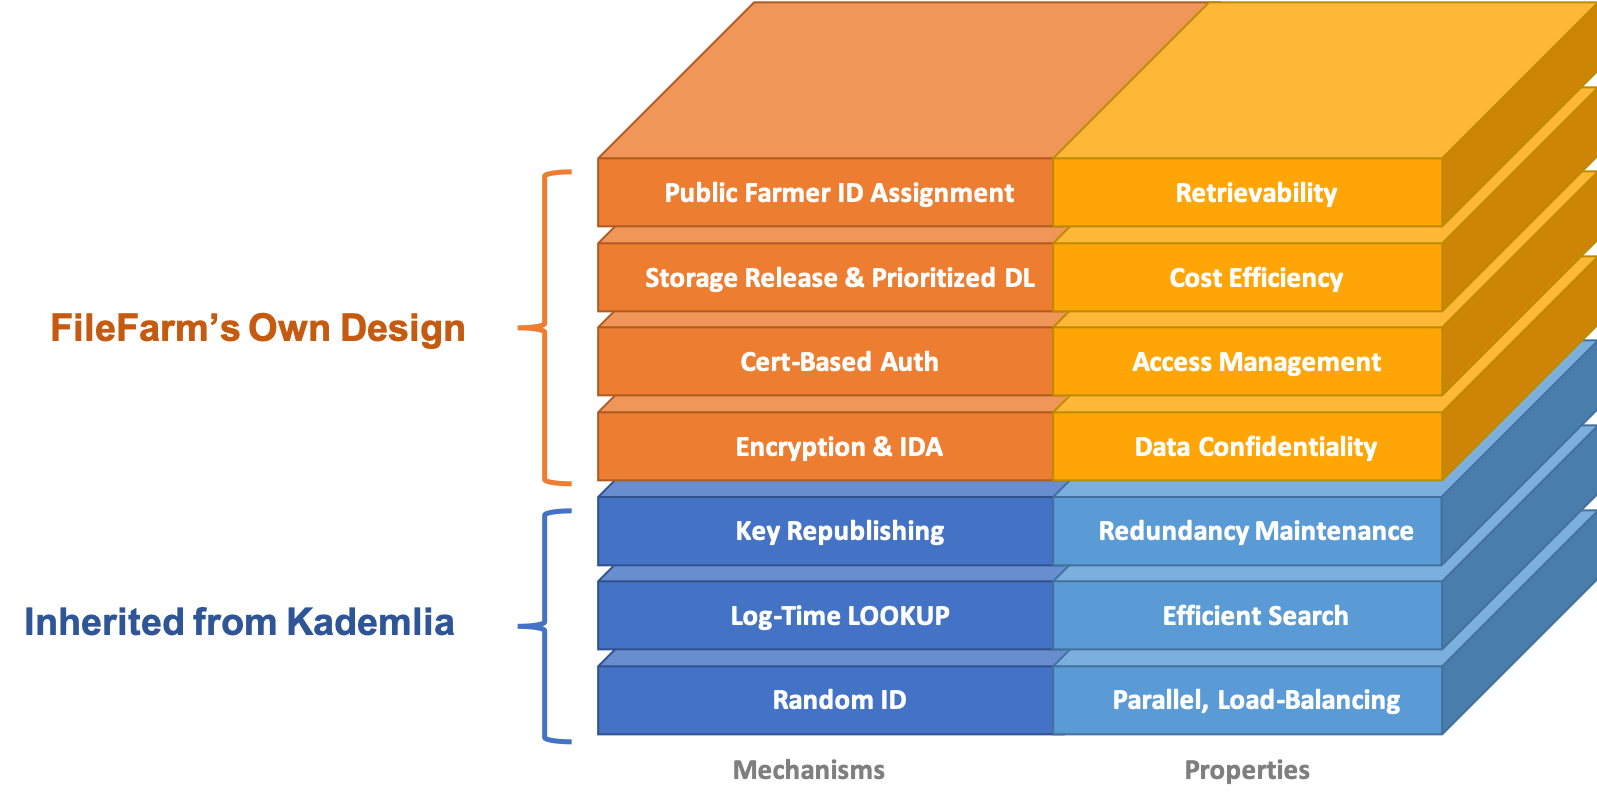
\includegraphics[width=14cm]{figures/property_stack.png}
  \caption{FileFarm's property stack}
  \label{fig:propertystack}
\end{figure}

\newpage

% data confidentiality
\section{Data Confidentiality}
\label{s:dataconfidentiality}

Designed to be a general-purposed P2P content sharing overlay, vanilla Kademlia protocol does not provide features of encryption and dispersion since data are meant to be shared instead of being kept in secret in most P2P applications. Thus, without confidentiality design, files will be uploaded to Kademlia network directly and the storing nodes will be able to peek content of the files. However, as FileFarm is a private storage system targeting on preserving data security and privacy, the mechanisms considering data confidentiality must be designed.

In order to preserve privacy and confidentiality while storing data on public clouds, FileFarm introduces a pre-processing flow of files before they are actually uploaded, in a sense that every files are randomly dispersed over clouds, and only the owner holds the key to retrieving and reconstructing them. To be precise, an example is shown in Figure \ref{fig:dataconfidentiality}. A file $F$ of size $S$ is sliced into chunks $C1, C2, ..., Cn$ of size $\frac{S}{n}$ and then chunks are encrypted into $E1, E2, ..., En$ of the same size, respectively. For each of the encrypted chunk, a \textit{sharding} process is performed based on an Information Dispersal Algorithm of $(p,q)$ schema (see \ref{s:informationdispersalalgorithm}), which produces $(p + q)$ shards of size $\frac{S}{n}*\frac{p+q}{p}$, and the original encrypted chunk can be recovered from any $p$ of these $p + q$ shards. Now the pre-processing flow is finished, and the $n * (p + q)$ generated shards are uploaded to FileFarm in parallel.

\begin{figure}[!b]
  \centering
    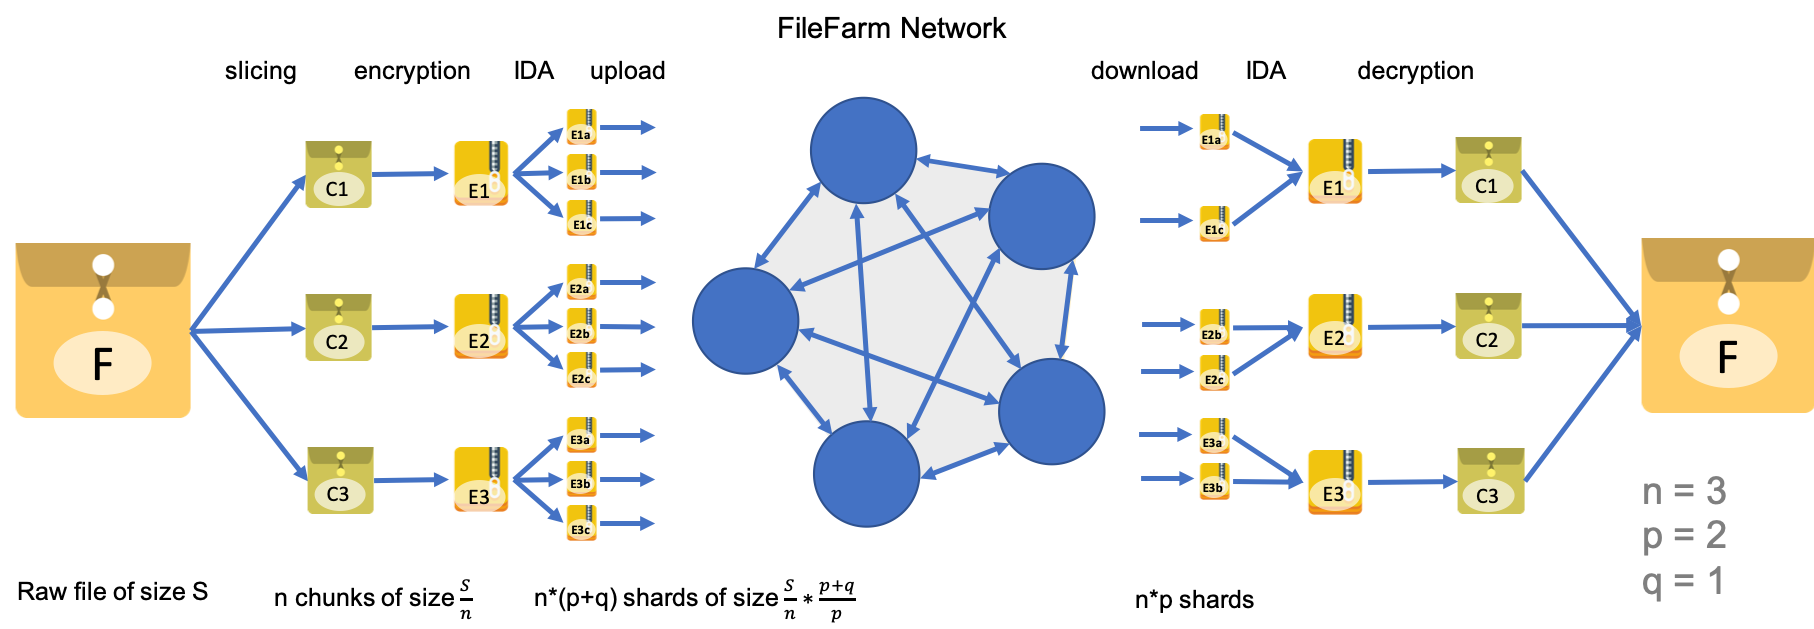
\includegraphics[width=15cm]{figures/data_confidentiality.png}
    \caption{An example of encryption and sharding flow}
    \label{fig:dataconfidentiality}
\end{figure}

\newpage

To reconstruct the original file $F$, the procedure seems inverted. For each of the encrypted chunks $E1, E2, ..., En$ that was sharded into $p+q$ shards, the client sends parallel requests to collect $p$ shards so that it can be reconstructed by IDA. The reconstructed chunks are then decrypted to $C1, C2, ..., Cn$ and combined into the original file, $F$.

% access management
\section{Access Management}
\label{s:accessmanagement}

Different from general P2P applications, FileFarm is an enterprise storage system applied in a \textbf{private} context. In such usage scenario, how to grant access to authorized users while denying connections from unauthorized ones plays a crucial role in security of the system. To achieve this goal, FileFarm adopts a decentralized approach toward access management. Different from common web systems, the access management design in FileFarm does not involve a centralized key directory. Instead, the account and key information is saved distributed-ly in FileFarm storage network, just like normal data, which means the access management mechanism has no dependence on any single farmer, and no data leakage will occur even if any farmer is compromised.

\newpage

\subsection{Decentralized Authentication}
\label{ss:decentralizedauthentication}

\begin{figure}[hbt]
  \centering
    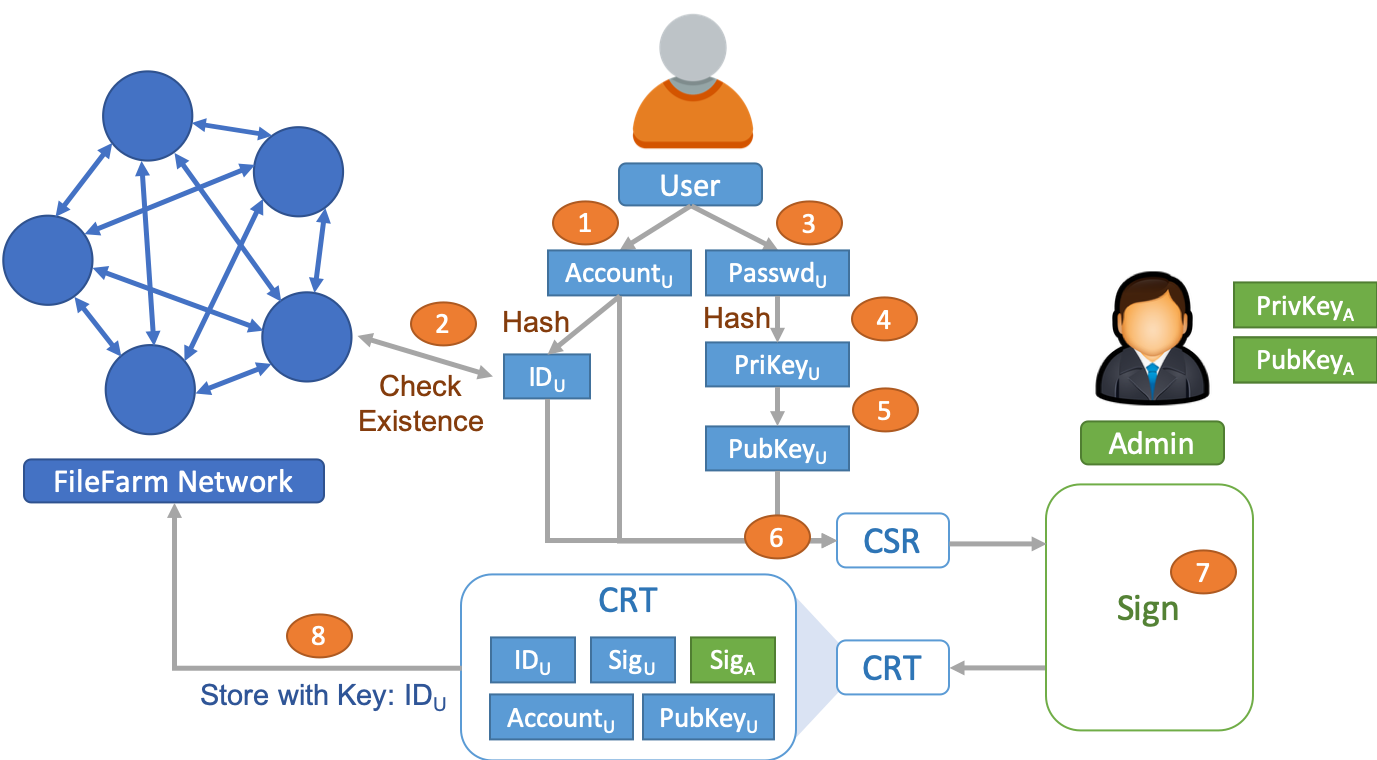
\includegraphics[width=14cm]{figures/access_management_register.png}
    \caption{An illustration of register procedure}
    \label{fig:accessmanagementregister}
\end{figure}
  
\begin{figure}[!b]
  \centering
    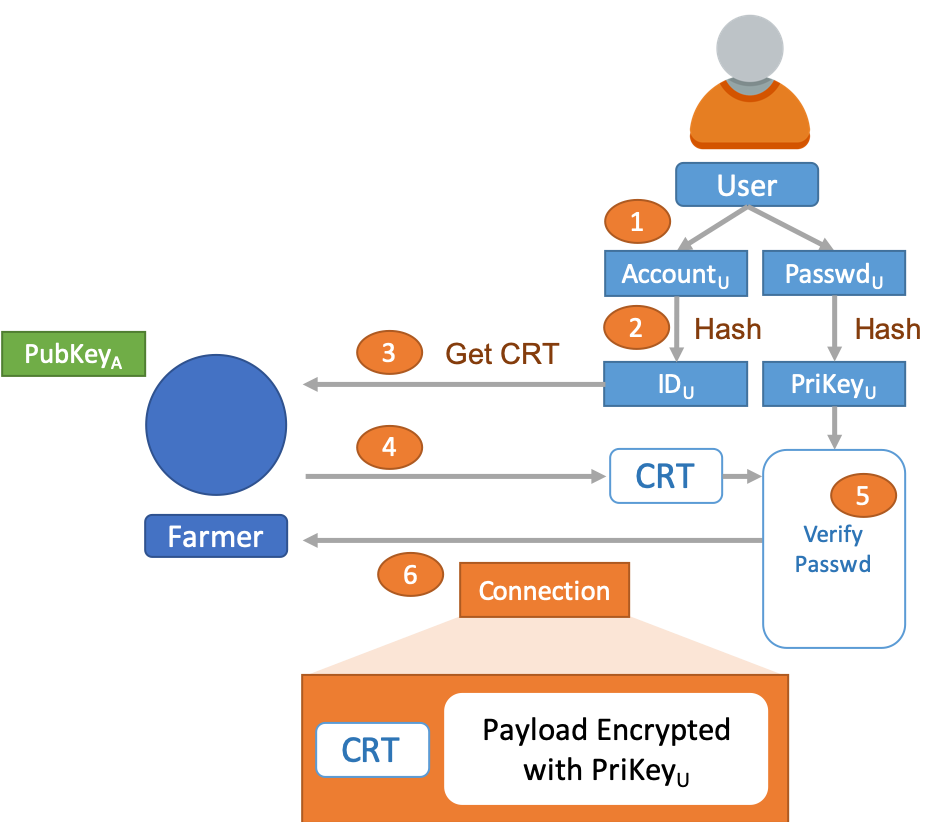
\includegraphics[width=12cm]{figures/access_management_login.png}
    \caption{An illustration of login procedure}
    \label{fig:accessmanagementlogin}
\end{figure}

\newpage

The decentralized authentication mechanism involves 2 major parts: (1) \textit{register}, (2) \textit{login}.

\begin{enumerate}
  \item \textbf{Register}: This process occurs when a user accesses the FileFarm system for the first time. From user's point of view, the goal of this process is to create an account, get permission from the administrator and then save account information into the network so that it can be accessed successfully next time, probably from a different client machine. This approach is based on the concept of Public Key Infrastructure, which is described in \ref{s:publickeyinfrastructure}, whereas the goal here is to validate clients but not serving hosts. The approach involves 3 roles: an administrator, the FileFarm cloud, and a user accessing FileFarm through a client application. To register an account, the user determines an account name($Account_{U}$) and a password ($Passwd_{U}$) in the client application. The account name and password will be hashed into user ID ($ID_{U}$) and private key ($PriKey_{U}$), respectively. The client application then checks existence of the account name by querying from the FileFarm cloud with user ID. If the account has not been registered yet, the procedure goes on. Client application will wrap (1) account name, (2) user ID, (3) user information, (4) a public key ($PubKey_{U}$) generated from user's private key and (5) a user's signature ($Sig_{U}$) into a certificate request (CSR). On receiving such request, the administrator makes a decision on whether to grant access for the client or not. If the client passes administrator's validation, the administrator creates a signature ($Sig_{A}$) on the signing request, which turns into a certificate. The certificate is then sent back to the client. When receiving a valid certificate, the client application stores it on the FileFarm cloud with key being her user ID, and the registration process is finished successfully.
  
  \newpage

  \item \textbf{Login}: This process is designed for a registered user to login to his account with account name and password, which are the only information needed to be carried by the user. The user can login via a client machine different from the one he used to register account. To login to FileFarm, the user first types account name ($Account_{U}$) and password ($Passwd_{U}$) into the client interface. The account name and password are hashed into user ID ($ID_{U}$) and private key ($PriKey_{U}$), respectively. Then the client application makes a query for the user's certificate from the FileFarm cloud. On receiving the certificate, the client verifies user's password by checking the signature on it. If the password validation succeeds, the client is allowed to access the FileFarm storage network. To access FileFarm, the client appends its certificate to the connection request packet, and then encrypts the payload with its own private key. When receiving request from clients, a farmer check the validity of the certificate by verifying the signature on it using administrator's public key. The farmer also verifies client's identity by decrypting the payload using client's public key specified in the certificate.
\end{enumerate}

\newpage

% cost efficiency
\section{Cost Efficiency}
\label{s:costefficiency}

FileFarm is built on the top of both public clouds and private premises. Storage fees are charged by public storage provider but not by the enterprises' own servers. Due to this fact, any storage operation executed on public clouds needs to be carefully inspected, in order to minimize the fee charged by public storage providers without lost of retrievability. As depicted in \ref{table:cloudstoragecost}, there are 2 major kind of storage fees: (1) \textit{static storage fee} per-GB / per-month (2) \textit{data transfer out fee} per-GB of download traffic. We will explain how the redundant fee comes from the original design and introduce the mechanism employed by FileFarm to reduce these fees in the following sub-sections.

\newpage

\subsection{Storage Release}
\label{ss:storagerelease}

The \textit{storage release} mechanism reduces \textit{static storage fee} by releasing unused redundant copies of shard and keeping redundancy at \textit{exactly K} but not more. To understand why there might be unused redundant copies of shard, we need to take a look at how the underlying Kademlia DHT protocol maintains redundancy.

As described in \ref{ss:redundancymaintenance}, Kademlia implements an \textit{Efficient Key Republishing} mechanism that ensures each shard will always have "at least" $K$ copies over the storage network. However, there are certain scenarios making number of copies more than $K$, which results in unneeded storage overhead. Considering a scenario in which a shard is kept by $K$ farmers and one of them churns off accidentally. With efficient key republishing, one of the remaining $K-1$
farmers will detect this and send a copy of the shard to the $K+1^{th}$ closest farmer, so that redundancy recovers from $K-1$ to $K$. However, when the failed farmer recovers from service outage, the redundancy will raise from $K$ to $K+1$. The copy on the $K+1^{th}$ closest farmer is now an unused overhead that need to be eliminated in order to save static storage cost.

This is the moment that storage release mechanism should work. Due to the fact that republishing message will only be sent to the $K$ closest farmers, the $K+1^{th}$ closest farmer will not receive this message, which triggers it to republish the shard in the next period. To find the $K$ closest farmers to this shard, a NODE\_LOOKUP procedure should be performed before sending republishing messages. This gives the $K+1^{th}$ closest farmer a chance to find itself not being one of the K closest farmers, it then stops the republishing process and deletes the shard from its storage. This shows the entire working procedure for storage release mechanism.

From the explanation above, we make a brief conclusion that \textit{storage release} is a mechanism that minimizes \textit{static storage fee} by holding redundant copies of each shard at exactly $K$ but not more. Besides, as the $K$-redundancy guideline still holds, \textit{storage release} does not induce retrievability concerns.

\newpage

\subsection{Prioritized Download}
\label{ss:prioritizeddownload}

\textit{Prioritized download} is a mechanism aiming to minimize the \textit{data transfer out} fee from public clouds. This mechanism only makes sense in hybrid cloud settings, where not only public clouds but also enterprise's private storage machines such as NAS or SAN are contributed to the storage system. Without \textit{prioritized download} mechanism, each farmer is treated equal and shares the same probability of serving data for clients. However, the cost of downloading data from public clouds is significantly higher than that of downloading from private servers, because of the \textit{data transfer out fee} charged by storage providers. \textit{Prioritized download} is the mechanism ensuring that shards are preferred to be downloaded from private farmers, so that \textit{data transfer out fee} is minimized.

In hybrid-cloud settings, enterprises optionally build their own private farmers. The private farmers are usually not as reliable as public ones. However, they have advantages in at least 2 aspects:

\begin{enumerate}
  \item High throughput and low delay in local area network (LAN)
  \item No data transfer fee needed
\end{enumerate}

These advantages make it reasonable for enterprises to split a portion of budgets on investment of private storage devices. This not only reduces data transfer fee charged by public clouds, but also improves download performance.

To understand how prioritized download works, we need to take a closer look at how the underlying Kademlia DHT protocol retrieves a shard. As described in \ref{ss:efficientsearch}, Kademlia implements an iterative VALUE\_LOOKUP procedure to retrieve shards. The VALUE\_LOOKUP procedure finishes immediately when any of the visiting farmers does store the shard, and the client will download the shard from that farmer.

\newpage

Prioritized download is a modified version of VALUE\_LOOKUP, with some noticeable differences:

\begin{enumerate}
  \item Prioritized download finishes once the target shard is found on a \textbf{private} farmer.
  \item Prioritized download memorizes a public farmer who has the shard when finding such one, but not download from it immediately.
  \item Prioritized download downloads from a public farmer only if there is no private farmer found storing the target shard
\end{enumerate}

By applying these differences to the VALUE\_LOOKUP procedure, \textit{prioritized download} ensures that shards will be downloaded from public farmers only if there is no private farmer serving the same shard. This effectively minimizes the data traffic flowing out from public clouds and also the \textit{data transfer out fee} charged by storage providers. Since \textit{prioritized download} only changes the preference of downloading order, any public farmer serving the shard will eventually be chosen once ther are no private farmers serving the same shard. This implies that \textit{prioritized download} does not affect retrievability of files.

From the description above, we know that FileFarm treats public farmers and private farmers differently. In fact, a special approach is implemented by FileFarm to achieve this kind of differentiation. We will explain the details and the benefits brought by such differentiation in \ref{ss:publicfarmeridassignment}.

\newpage

% retrievability
\section{Retrievability}
\label{s:retrievability}

In FileFarm's design, redundancy introduced by the $K$ factor of Kademlia (\ref{s:kademlia}) and the $q$ factor of information dispersal algorithm (\ref{s:informationdispersalalgorithm}) both contribute to retrievability of files. However, considering a hybrid-cloud case in which some shards are stored totally on private farmers but no public ones. The significant reliability difference between public and private farmers would cause a large disparity in retrievability of files, which makes the system's behavior unpredictable. To provide a more rigorous guarantee on retrievability in hybrid-cloud settings where reliability of public clouds and private servers differs greatly, we have to make sure every shards are saved on at least 1 public cloud with high probability. This demand gives rise to the design of \textit{public farmer ID assignment}.

\subsection{Public Farmer ID Assignment}
\label{ss:publicfarmeridassignment}

To differentiate public farmers from private ones, FileFarm gives public farmers a special identity. In the 160-bit farmer ID space, each public farmer is assigned with an ID with last 144 bits be '0', hence there can be at most $2^{16}=65536$ public farmers in the network. In contrast, ID of private farmers are generated randomly but cannot have last 144 bits be '0'. Besides, public farmer IDs are issued in bit-reversal permutation ordering. To be clear, we explain this kind of ordering in a simplified case where public IDs vary in the first 4 bits and have last 156 bits be '0' (see figure \ref{fig:bitreversalpermutationordering}). To generate ID for the $i^{th}$ public farmer, we reverse the binary representation of the number $i-1$ and assign the resulting binary string as the first 4 bits of the newly-generated ID. Following this rule, the first 4 bits of generated public IDs will be '0000', '1000', '0100', '1100', ...

With public farmer IDs being assigned in bit-reversal permutation ordering, we can be certain that public farmers are dispersed over the 160-bit ID space. Since that hash value of shards follow a uniform distribution over the 160-bit key space and that shards are stored on farmers with ID closest to its hash value, the dispersion of public farmer IDs makes them load-balanced in terms of storage usage and request frequencies. Besides, this explicit assignment also avoids the situation that public farmer's IDs distribute uneven over the network, which would cause disparity between retrievability of shards.

To sum up, the assigning rule of public farmer ID brings following benefits:

\begin{enumerate}
  \item Provides an explicit rule to distinguish public farmers from private ones, which is needed for prioritized download (\ref{ss:prioritizeddownload}) to work.
  \item Poses a strong guarantee on load-balancing of public farmers, which in further minimizes the reliance on any single public cloud.
  \item Maximizes the likelihood of each shard to be stored by at least one public farmer, which improves the average retrievability of each shard and thus enhances the overall retrievability of files.
\end{enumerate}

\begin{figure}[!b]
\centering
  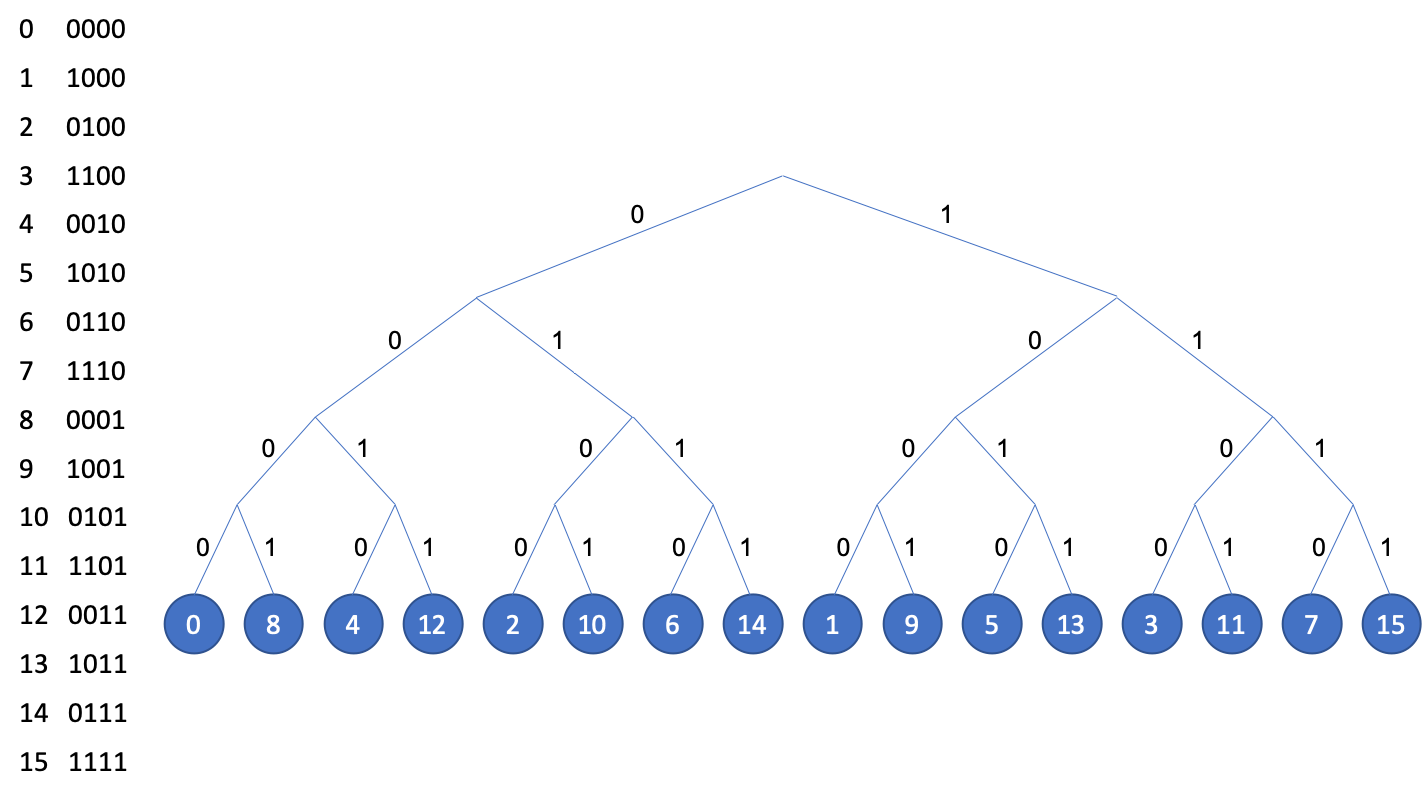
\includegraphics[width=15cm]{figures/bit_reversal_permutation_ordering.png}
  \caption{Bit-reversal permutation ordering with prefix length = 4}
  \label{fig:bitreversalpermutationordering}
\end{figure}
\chapter{Experiments and Results}
\label{c:experiments_and_results}

To verify the claimed properties of FileFarm, we conduct a series of experiments. In this chapter, we will describe our experimental environment first, and then describe settings, process, and results of each experiments.

% Environment
\section{Environment}
\label{s:expenvironment}

In the following experiments, we run FileFarm on 5 physical hosts with following system information:

\begin{itemize}
    \item CPU: Intel(R) Xeon(R) CPU E5-1630 v3 @ 3.70GHz
    \item Memory: 16 GiB DDR4
    \item Network Interface: Ethernet Connection (2) I218-LM (1Gbit/s)
    \item Operating System: Ubuntu Server 18.04.2 LTS
\end{itemize}

 \noindent Each of the 5 physical hosts is assigned with a static IP address, and all of the 5 IP addresses belong to the same subnet with mask 255.255.255.0. Depending on settings of each experiment, a physical host might runs one or multiple instances of FileFarm farmers and clients simultaneously.

\newpage

% exp: NODE_LOOKUP Efficiency
\section{Experiment: NODE\_LOOKUP Efficiency}
\label{s:expnodelookupefficiency}

In FileFarm, each shard is stored on exactly $K$ farmers. Instead of saving location of shards as static records in a centralized database, FileFarm adopts Kademlia's dynamical lookup procedures. Thus, the efficiency of these procedures will impact system's I/O performance greatly. According to the sketch of proof in \cite{maymounkov2002kademlia}, NODE\_LOOKUPs in a Kademlia network will finish in $\lceil log(n) \rceil + c$ steps for some small constant of $c$, where $n$ is network size, i.e., number of nodes in the network. We want to verify that this property also holds in FileFarm.

In this experiment, we start $m$ farmers on each physical host; thus there are $n = 5 \times m$ farmers in total. After all farmers are bootstrapped, we make each farmer NODE\_LOOKUP 10 random targets and report the number of hops needed to locate the $K$ closest farmers around the target. Then we collect and compute mean of hops needed. The whole process is repeated for $m=1,2,5,10,20,50$ and $K=1,2,3,4,5$.

\begin{figure}[hbt]
\centering
  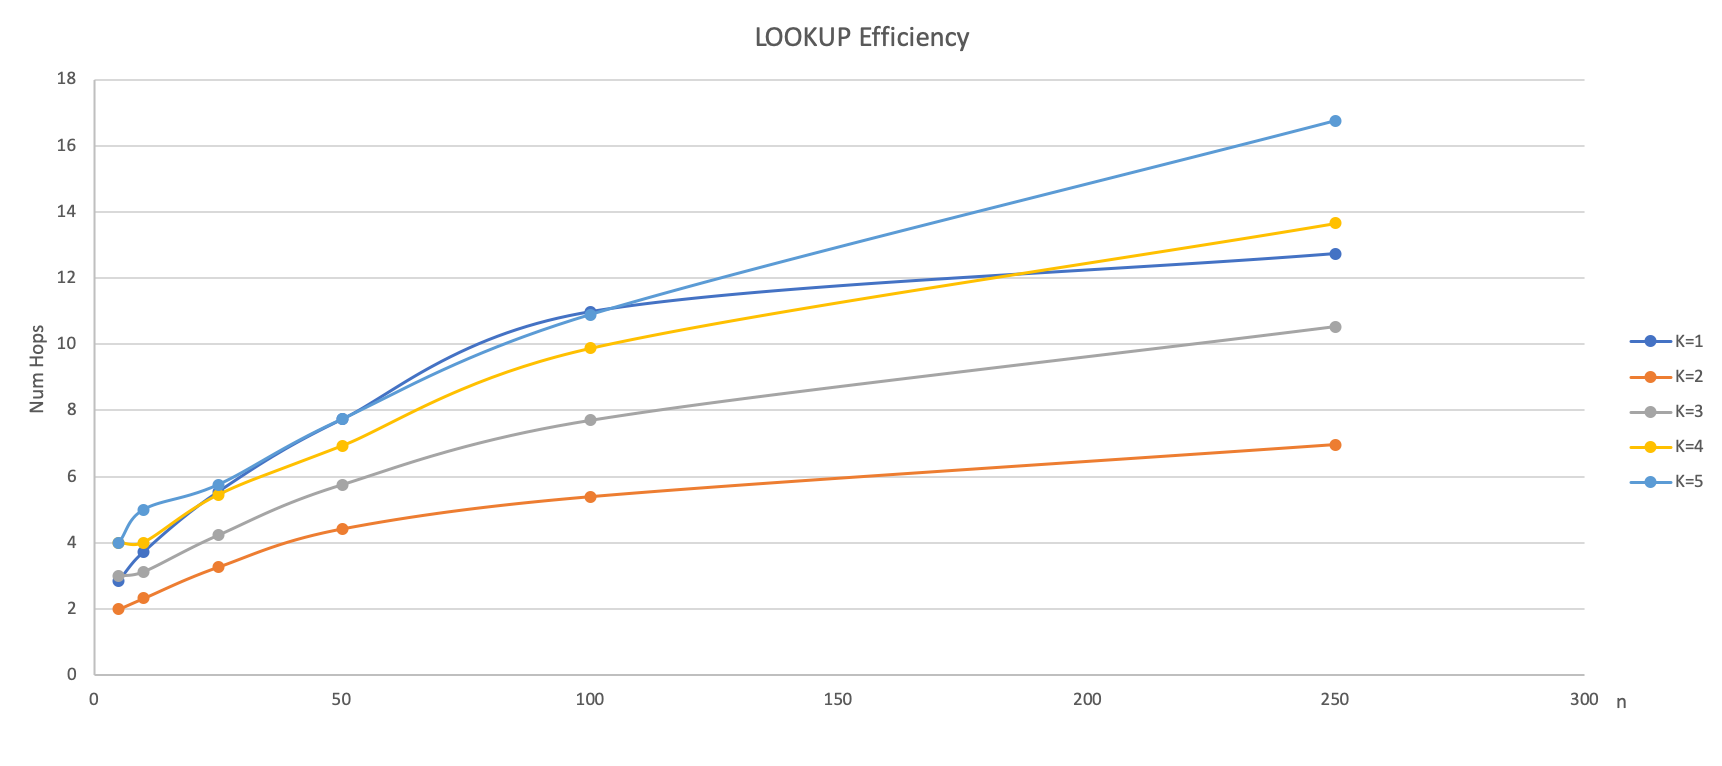
\includegraphics[width=14cm]{charts/chart_lookup_efficiency.png}
  \caption{Number of NODE\_LOOKUP steps (hops) with respect to $K$ and network size}
  \label{fig:lookupefficiency}
\end{figure}

From Figure \ref{fig:lookupefficiency}, we can observe that number of NODE\_LOOKUP steps grows with number of farmers, following a logarithm-like curve. With number of farmers growing from 100 to 200, it only takes around 2 more steps to locate all $K$ closest farmers, which makes FileFarm network scalable. However, it can also be observed that a larger setting of $K$ requires more steps for NODE\_LOOKUP procedure to finish, which is intuitive, considering the fact that NODE\_LOOKUP finds all of the $K$ closest farmers but not one or some of them.


% exp: VALUE_LOOKUP Efficiency
\section{Experiment: VALUE\_LOOKUP Efficiency}
\label{s:expvaluelookupefficiency}

Just like performing NODE\_LOOKUP before uploading a shard, farmers perform VALUE\_LOOKUP before downloading a shard. Different from NODE\_LOOKUP, the VALUE\_LOOKUP procedure finishes immediately when the target value is found. Thus, VALUE\_LOOKUP procedure only needs to reach any one of the $K$ closest farmers instead of finding all of them. According to Cai's analysis\cite{cai2013probabilistic}, it takes no more than $(1+O(1))\frac{log(n)}{H_{K}}$ steps for any node in a Kademlia network to locate any other node, where $H_K = \sum_{i=1}^{K} 1/i$. This upper bound also stands for VALUE\_LOOKUP, considering the fact that VALUE\_LOOKUP for the target key converges along the same path as NODE\_LOOKUP for the closest farmer, due to $unidirectionality$ of XOR distance metric. In this experiment, we want to verify this property on FileFarm and compare the result with \ref{s:expnodelookupefficiency}.

In this experiment, we start $m$ farmers on each physical host; thus there are $n = 5 \times m$ farmers in total. After all farmers are bootstrapped, we starts 1 client on each physical hosts and make them upload 100 random files in total. Then we make each client send 200 file download requests randomly and let farmers report the number of hops needed for each VALUE\_LOOKUP. We collect and compute mean of hops needed. The whole process is repeated for $m=1,2,5,10,20,50$ and $K=1,2,3,4,5$.

\begin{figure}[hbt]
\centering
  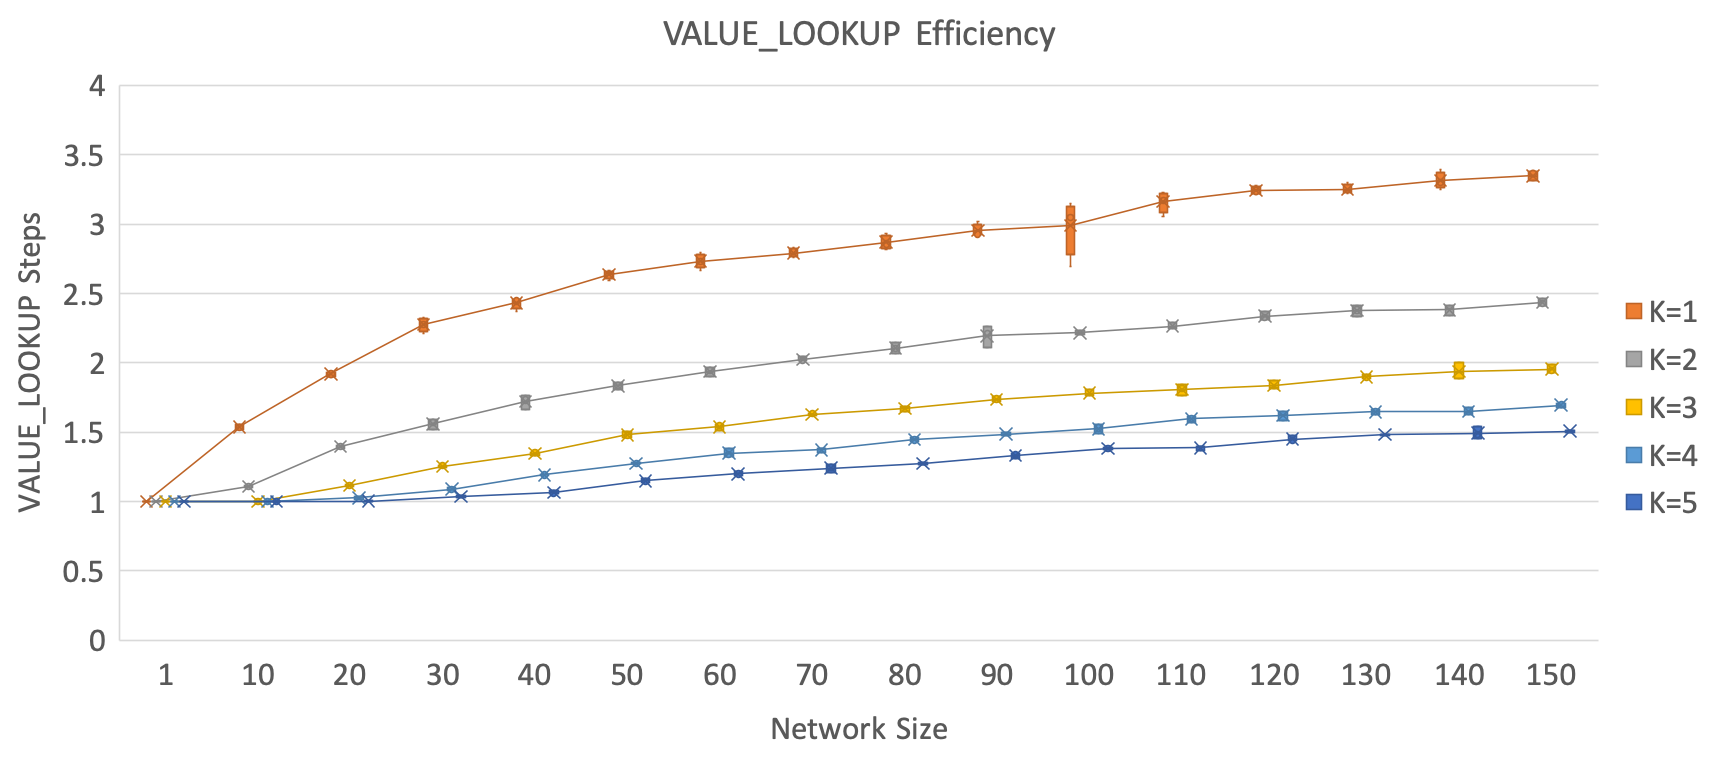
\includegraphics[width=14cm]{charts/chart_value_lookup_efficiency.png}
  \caption{Number of VALUE\_LOOKUP hops with respect to $K$ and network size}
  \label{fig:valuelookupefficiency}
\end{figure}

\newpage

From figure \ref{fig:valuelookupefficiency}, we can observe that VALUE\_LOOKUP also follows a logarithm curve, but the number of hops needed is far less than that needed by NODE\_LOOKUP shown in \ref{fig:lookupefficiency}. In a FileFarm network of 100 farmers, it only takes less than 3 hops to find a shard. Besides, as $K$ increases, number of hops decreases roughly with a factor $H_{K}$ depicted by Cai\cite{cai2013probabilistic}. Putting this result with \ref{s:expnodelookupefficiency}, we can conclude that a larger choice of $K$ results in more uploading overhead, while improves download performance.

% exp: Retrievability
\section{Experiment: Retrievability}
\label{s:expretrievability}

Retrievability is one of the most important metrics used to measure quality of a cloud storage system. In this experiment, we want to examine how FileFarm is likely to keep client's data, and how certain configuration parameters affect the likelihood of uploaded files to be retrievable by clients. To be precise, we define retrievability as:

\begin{center}
  $Retrievability = \frac{\# Successfully Reconstructed}{\# Total Download Attempts}$
\end{center}

\noindent Belows are the configuration parameter to be considered in this experiment:

\begin{enumerate}
  \item $\alpha$: Online probability of each farmer.
  \item $K$: Number of redundant copies stored for each shard.
  \item $q$: Redundancy parameter in a (4, q) IDA schema; A file is recoverable given any 4 out of the (4+q) shards.
\end{enumerate}

As for the experimental procedure, we runs 10 farmers with online probalility $\alpha$. After the farmers are bootstrapped, we run 100 clients and make them start random uploading/downloading. For each download request, the client reports if the file is successfully reconstructed. We Collect 1,000,000 reports from clients and compute retrievability. The whole process is repeated for $K=1,2,3$, $q=0,1,2$ and $\alpha=0.9,0.99$.

\begin{table}[hbt]
  \centering
    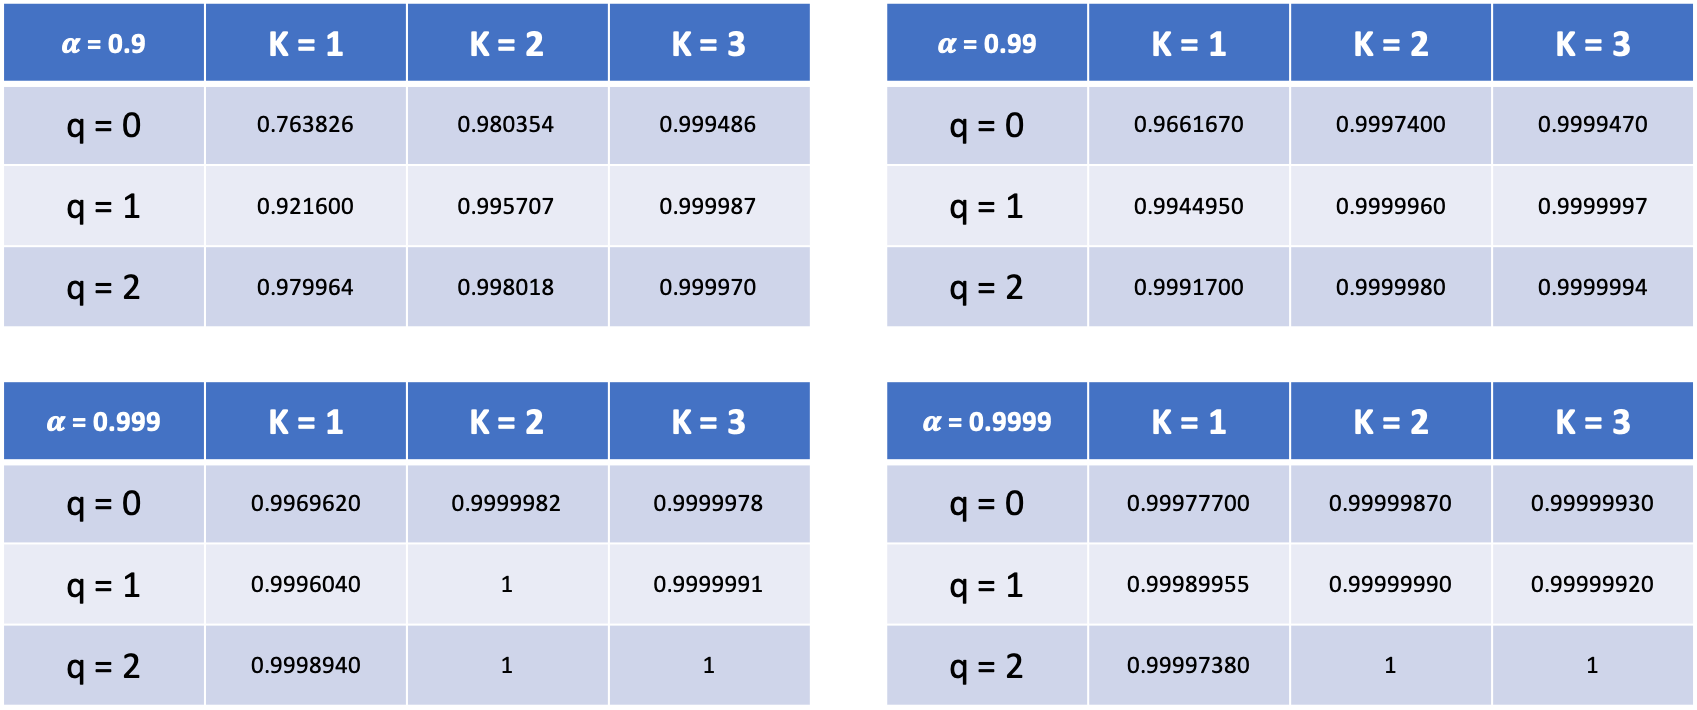
\includegraphics[width=14cm]{tables/table_retrievability.png}
    \caption{Retrievability of files with respect to $\alpha$, $K$ and $q$}
    \label{table:retrievability}
\end{table}
  
\begin{figure}[hbt]
  \centering
    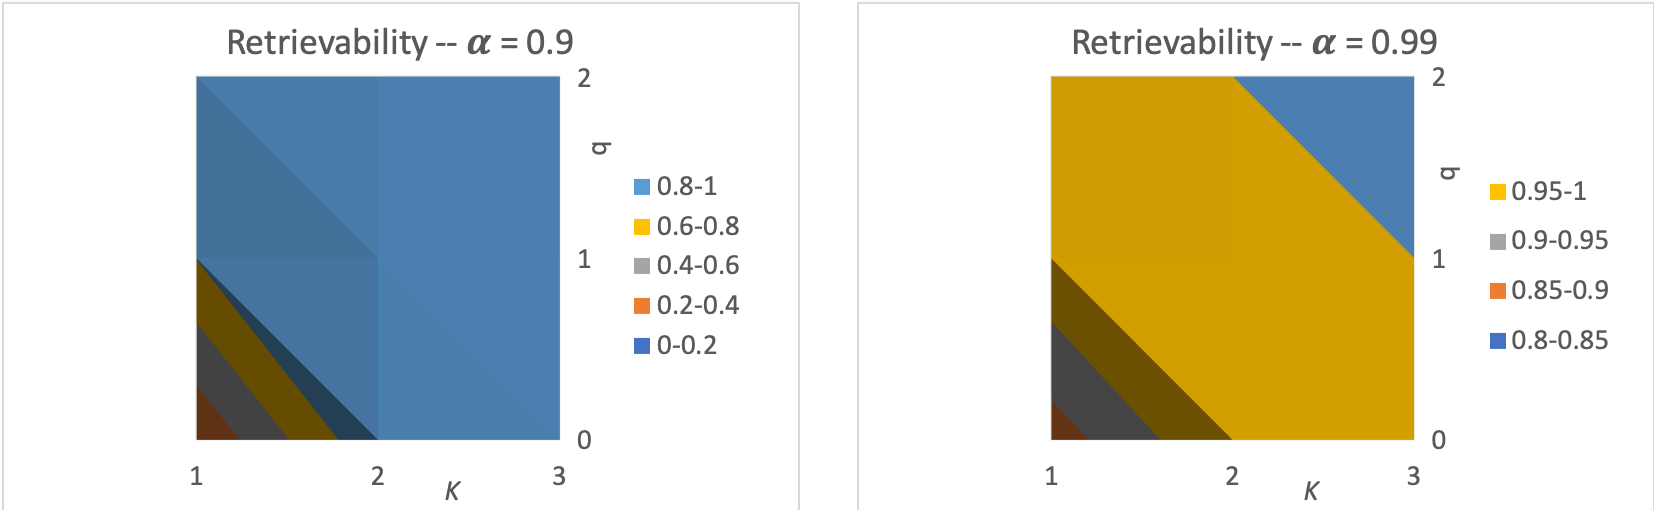
\includegraphics[width=14cm]{charts/chart_retrievability.png}
    \caption{Retrievability of files with respect to $\alpha$, $K$ and $q$}
    \label{fig:retrievability}
\end{figure}

From the result shown in \ref{table:retrievability}, we observe that network redundancy parameter $K$ and IDA redundancy parameter $q$ both effectively impact the retrievability of files. By increasing $K$, retrievability can be improved significantly. However, increasing $K$ has a relatively large overhead, considering the fact that an incremental in $K$ will consume an extra amount of storage space equaling to the actual file size. To reduce cost while preserving retrievability, increasing $q$ is a resonable choice. In addition, we also observe that a selection of $K=2$ roughly squares the data lost probability. For example, within a system where farmers have $0.1$ probability to be offline, a setting of $K=2 and q=1$ roughly achieves the data lost rate of $0.1^{2}=0.01$, which is effective considering the fact that a cloud service normally has much lower probability to be unavailable, and we can make the probalility of losing data even lower by building FileFarm upon them.

\newpage

% exp: Throughput
\section{Experiment: Throughput}
\label{s:expthroughput}

In this experiment, we want to test FileFarm's I/O performance under different file size and sharding schemes. As described in figure \ref{fig:uploadflow} and figure \ref{fig:downloadflow}, the upload process of FileFarm involves slicing, encryption, IDA computation, NODE\_LOOKUP, ... while the download process involves VALUE\_LOOKUP, IDA computation, decryption, combining... Some operations can be done in parallel, while others cannot. To analyze performance of such complicated flows, we run experiments and measure the elapsed time.

As for the experimental procedure, we runs 5 farmers and 25 clients in total. Each farmer is assumed to have a 10 MB/s upload bandwidth. Once all farmers and clients are bootstrapped, we let clients start random upload and download files of size $S$ with a sharding scheme which generates $p$ shards in total. While uploading and downloading, we let clients report time consumption for each operations until 100 upload and 100 download reports have been collected. We collect these reports and compute mean of upload/download throughput. The whole process is repeated for $S=1,4,16,64,256,1024$ and $p=1,2,4,8,16,32$.

\begin{figure}[hbt]
\centering
  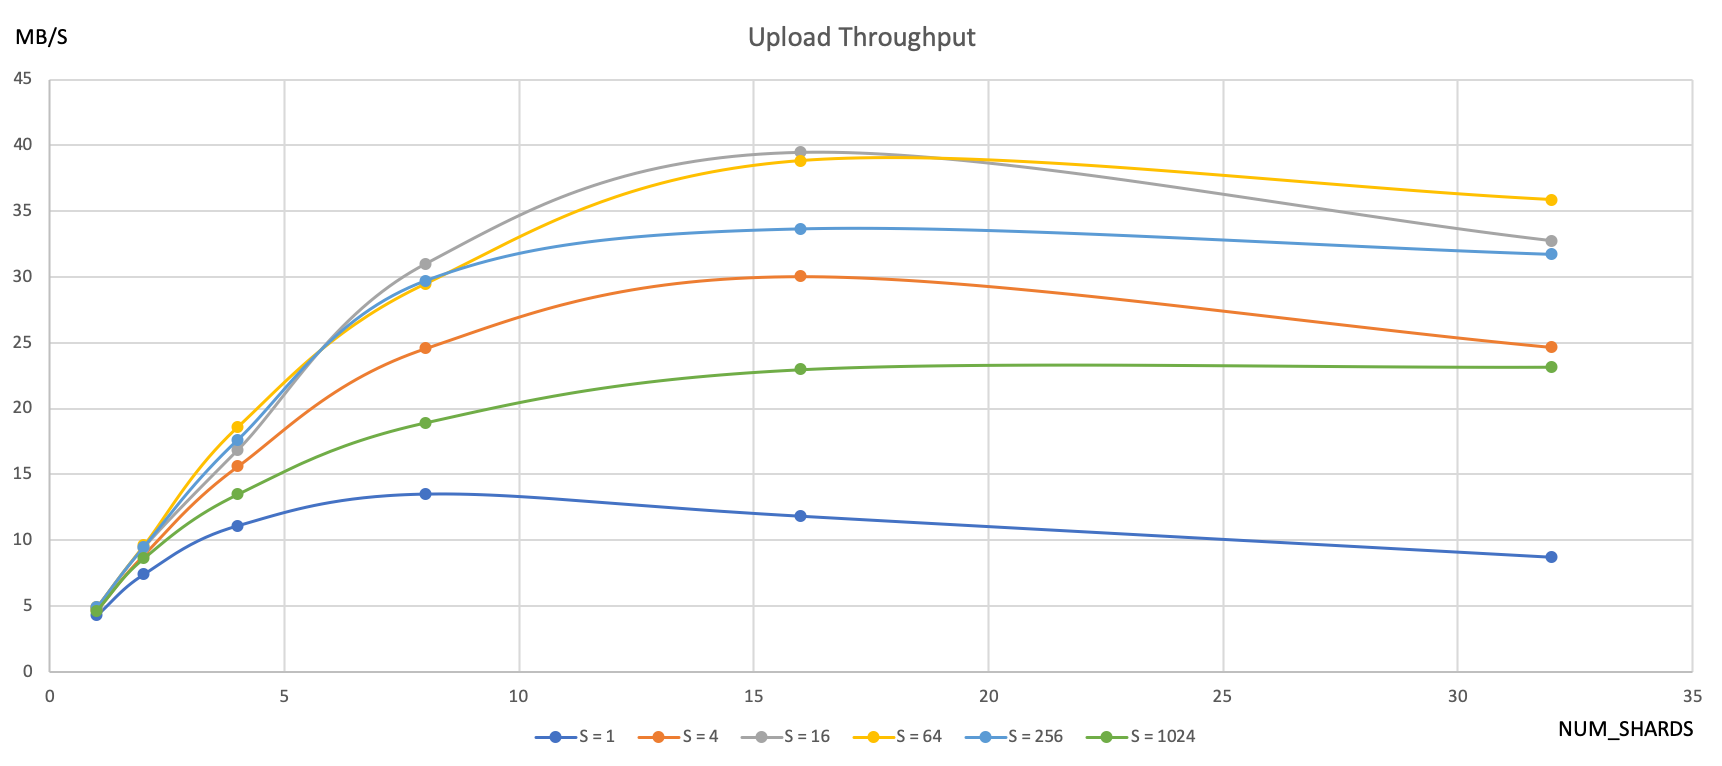
\includegraphics[width=14cm]{charts/chart_upload_throughput.png}
  \caption{Upload throughput with respect to file size and number of shards}
  \label{fig:uploadthroughput}
\end{figure}

\begin{figure}[hbt]
\centering
  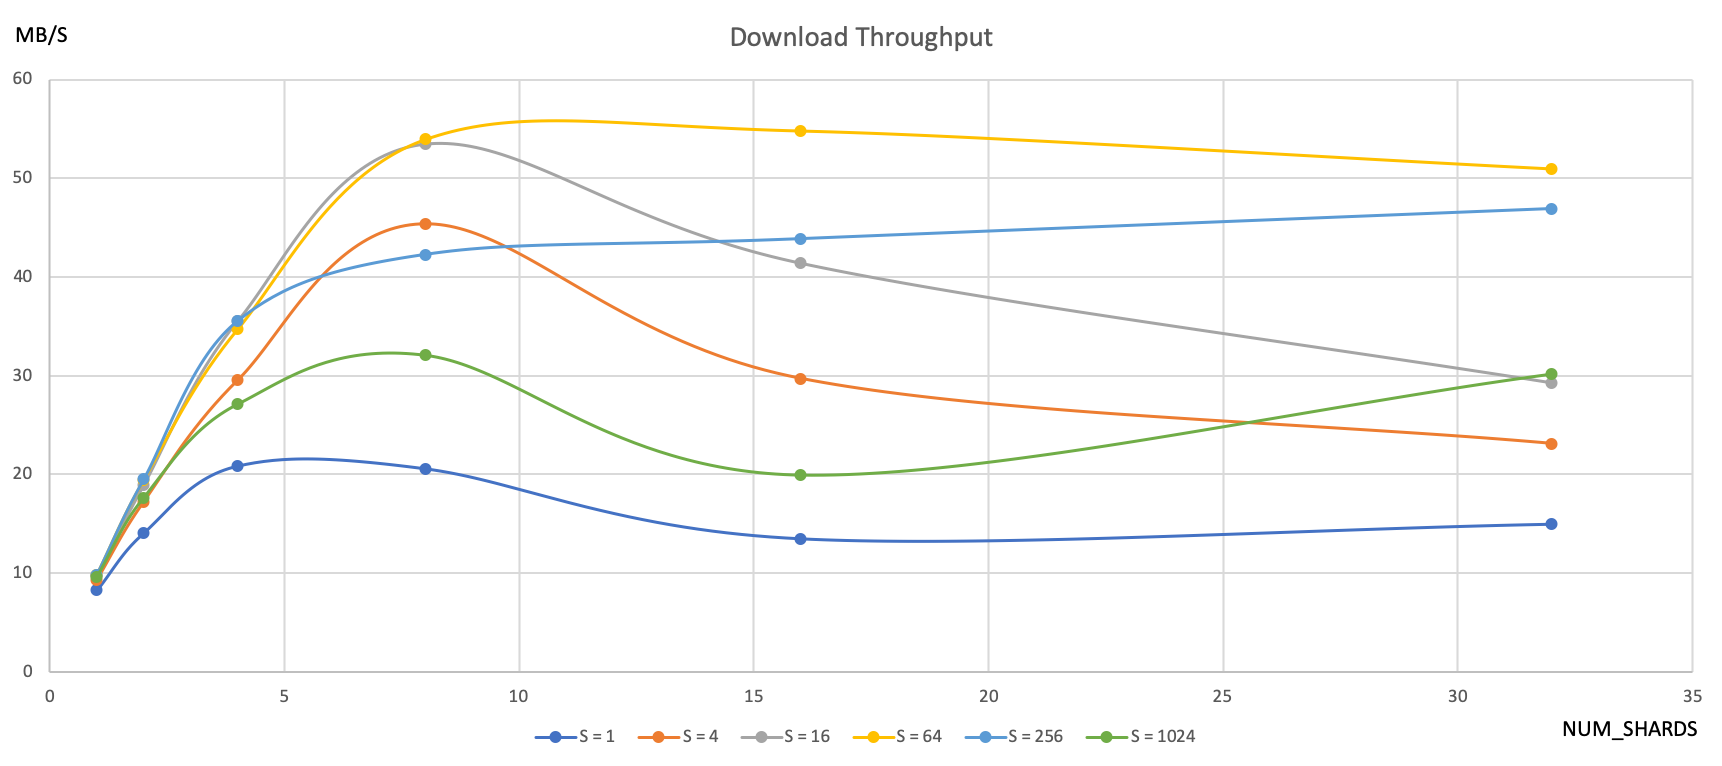
\includegraphics[width=14cm]{charts/chart_download_throughput.png}
  \caption{Download throughput with respect to file size and number of shards}
  \label{fig:downloadthroughput}
\end{figure}

From the result shown in figure \ref{fig:uploadthroughput}, we observe that uploading throughput grows when number of shards increases. This trends achieve peak value when number of shards = 16. After that, the curve goes down. With a file of size 64 MB, a sharding schema in which $p=16$ brings a best performance of around 39 MB/s.

Due to the procedural differences, the chart of download throughput, figure \ref{fig:downloadthroughput} seems different from that of upload throughput. First, the curves achieve peak value when number of shards is around 8. Second, download throughput is generally higher than upload throughput. This is because of the fact that download only involves retrieval of 1 copy of the target shard instead of $K$. Considering figure \ref{fig:uploadthroughput} and figure \ref{fig:downloadthroughput} collectively, we can conclude that under this scenario, choices of \#shards = 8 or 16 brings the best I/O performance in general.

% % exp: Cost Efficiency
% \section{Experiment: Cost Efficiency}
% \label{s:expcostefficiency}
\chapter{Conclusion}
\label{c:conclusion}

In this work, we propose FileFarm, a P2P overlay that leverages existing cloud services to form a secured cloud-of-clouds storage system with no single-point-of-failure. Beyond the desired properties inherited from Kademlia DHT such as load-balancing, efficient search and redundancy maintenance, FileFarm is provided with additional designs in order to meet requirements in various aspects: data confidentiality, access management, cost efficiency and retrievability. As a whole, FileFarm integrates these characteristics into a robust enterprise cloud storage system in terms of cloud-of-clouds or even a hybrid setting where enterprises' private servers cooperate with public clouds to offer services with lower delay and higher throughput. The benefits and overhead of our designs are explored by both analytical approaches and experiments. We also implement a prototype of FileFarm and evaluate performance or our novel P2P cloud storage solution based on it.

\appendix

\backmatter

\addcontentsline{toc}{chapter}{\bibname}
\bibliographystyle{abbrv}

% Your bibliography goes here
\bibliography{thesis}

\end{document}
